\documentclass[11pt]{beamer}
\usepackage[T1]{fontenc}
\usepackage{lmodern}
\usepackage[ngerman]{babel}
\usetheme{CambridgeUS}
\usepackage{amsthm}
\usepackage{amsmath}
\usepackage{amsfonts}
\usepackage{makeidx}
\usepackage{graphicx}
\usepackage{ragged2e}
\usepackage[list=true, font=large, labelfont=bf, 
labelformat=brace, position=top]{subcaption}
\usecolortheme{dolphin}
\usepackage{tcolorbox}
\usepackage[numbered,framed]{matlab-prettifier}
\usepackage{csquotes}
\usepackage{listings}
\usepackage{xcolor}
\usepackage{floatrow}
\usepackage{siunitx}
\usepackage{ragged2e}
\usepackage{booktabs}
\usepackage{newtxmath}

\lstset{literate=%
	{Ö}{{\"O}}1
	{Ä}{{\"A}}1
	{Ü}{{\"U}}1
	{ß}{{\ss}}2
	{ü}{{\"u}}1
	{ä}{{\"a}}1
	{ö}{{\"o}}1
}
\captionsetup{
	justification = centering
}
\newtcolorbox{mybox}{colback=red!2!white,colframe=red!75!black}

\newcommand{\norm}[1]{\left\lVert#1\right\rVert}
\newcommand{\N}{{\mathbb N}}
\newcommand{\R}{{\mathbb R}}
\newcommand{\C}{{\mathbb C}}
\newcommand{\Z}{{\mathbb Z}}
\newcommand{\Q}{{\mathbb Q}}
\newcommand{\coloneqq}{:=}
\newcommand{\hspf}{\hspace*{\fill}}
\newcommand{\Rd}{{\R^\text{d}}}
\newcommand{\Rdd}{{\R^{\text{d} \times }}}
\newcommand{\Diff}{\text{Diff}}
\newcommand{\totdeg}{\text{deg}_{tot}}
\newcommand{\F}[1]{\mathbb{F}_{#1}}
\newcommand{\Id}{\text{Id}}

\definecolor{Darkgreen}{rgb}{0.13, 0.55, 0.13}
\definecolor{Blue}{rgb}{0.0, 0.28, 0.67}
\definecolor{Purple}{rgb}{0.0, 0.28, 0.67}
\definecolor{Orange}{rgb}{1.00,0.67,0.00}
\definecolor{code}{rgb}{0.0, 0.0, 0.0}
\definecolor{Decorators}{rgb}{0.5,0.5,0.5}
\definecolor{Numbers}{rgb}{0.5,0,0}
\definecolor{MatchingBrackets}{rgb}{0.25,0.5,0.5}
\definecolor{Keywords}{rgb}{0,0.60,0.30}
\definecolor{self}{rgb}{0,0,0}
\definecolor{Strings}{rgb}{0.6,0.63,0}
\definecolor{Comments}{rgb}{0,0.63,1}
\definecolor{Backquotes}{rgb}{0,0,0}
\definecolor{Classname}{rgb}{0,0,0}
\definecolor{FunctionName}{rgb}{0,0,0}
\definecolor{Operators}{rgb}{0,0,0}
\definecolor{Background}{rgb}{0.98,0.98,0.98}
\definecolor{colKeys}{RGB}{0,0,255}       % blau
\definecolor{colIdentifier}{RGB}{0,0,0}   % schwarz
\definecolor{colComments}{RGB}{34,139,34} % gruen
\definecolor{colString}{RGB}{160,32,240}  % violett

\captionsetup[subfigure]{labelformat=brace, subrefformat=brace}
\renewcommand{\thesubfigure}{\arabic{subfigure}}

\lstset{%
	language=MATLAB,%
	basicstyle={\footnotesize\ttfamily},%
	breakautoindent=true,%
	breakindent=10pt,%
	breaklines=true,%
	captionpos=t,%
	columns=fixed,%
	commentstyle={\itshape\color{Darkgreen}},%
	extendedchars=true,%
	frame=single,%
	framerule=1pt,%
	identifierstyle={\color{colIdentifier}},%
	keywordstyle={\color{colKeys}},%
	keywordstyle=[2]\color{Orange},
	keywordstyle=[3]\color{Blue}\underbar,%
	morekeywords={%
		arguments,switch,case,otherwise,assert,clearvars,vpa,simplify,sym,scatter3%
	},%
	morekeywords=[2]{mustBeReal,mustBeMember,mustBeRealOrLogical,mustBeText,mustBeInteger,mustBePositive},% argumentchecks
	morekeywords=[3]{},%custom functions
	numbers=left,%
	numbersep=1em,%
	numberstyle={\tiny\ttfamily},%
	showspaces=false,%
	showstringspaces=false,%
	stringstyle={\color{colString}},%
	morestring=[d]{"},%
	tabsize=4,%
	xleftmargin=1em,%
	xrightmargin=1em%
}


\newtheoremstyle{indent}% name
{\topsep}%      Space above, empty = `usual value'
{\topsep}%      Space below
{\addtolength{\leftskip}{1.5em}}% Body font
{-1.5em}%         Indent amount (empty = no indent, \parindent = para indent)
{\bfseries}% Thm head font
{}%        Punctuation after thm head
{\newline}% Space after thm head: \newline = linebreak
{}%{\thmname{#1}\thmnumber{ #2}\thmnote{ #3}}%         Thm head spec

\newtheoremstyle{custom}% name
{\topsep}%      Space above, empty = `usual value'
{\topsep}%      Space below
{\addtolength{\leftskip}{1.5em}}% Body font
{-1.5em}%         Indent amount (empty = no indent, \parindent = para indent)
{\bfseries}% Thm head font
{}%        Punctuation after thm head
{\newline}% Space after thm head: \newline = linebreak
{}%{\thmname{#1}\thmnumber{ #2}\thmnote{ #3}}%         Thm head spec

\renewcommand{\thesubfigure}{\roman{subfigure}}

\newtheoremstyle{indent}% name
{\topsep}%      Space above, empty = `usual value'
{\topsep}%      Space below
{\addtolength{\leftskip}{1.5em}}% Body font
{-1.5em}%         Indent amount (empty = no indent, \parindent = para indent)
{\bfseries}% Thm head font
{}%        Punctuation after thm head
{\newline}% Space after thm head: \newline = linebreak
{}%{\thmname{#1}\thmnumber{ #2}\thmnote{ #3}}%         Thm head spec

\newtheoremstyle{custom}% name
{\topsep}%      Space above, empty = `usual value'
{\topsep}%      Space below
{\addtolength{\leftskip}{1.5em}}% Body font
{-1.5em}%         Indent amount (empty = no indent, \parindent = para indent)
{\bfseries}% Thm head font
{}%        Punctuation after thm head
{\newline}% Space after thm head: \newline = linebreak
{}%{\thmname{#1}\thmnumber{ #2}\thmnote{ #3}}%         Thm head spec

\renewcommand{\thesubfigure}{\roman{subfigure}}

%\renewcommand{\thesection}{\arabic{chapter}.\arabic{section}}

%\swapnumbers
\theoremstyle{custom}
\newtheorem{thm}{Theorem}[section]
%\renewcommand{\thetheorem}{\arabic{chapter}.\arabic{theorem}}
\newtheorem{proposition}[theorem]{Satz}
\newtheorem{lem}[theorem]{Lemma}
\newtheorem{cor}[theorem]{Korollar}


\theoremstyle{custom}
\newtheorem{dfn}[theorem]{Definition}
\newtheorem{conj}[theorem]{Vermutung}
\newtheorem{exm}{Beispiel}[section]
\newtheorem{exs}[exm]{Beispiele}

\newtheorem{remark}[theorem]{Bemerkung}
\newtheorem{remarks}[theorem]{Bemerkungen}
\newtheorem{nte}[theorem]{Notiz}
\makeatletter
\renewcommand*\env@matrix[1][\arraystretch]{%
	\edef\arraystretch{#1}%
	\hskip -\arraycolsep
	\let\@ifnextchar\new@ifnextchar
	\array{*\c@MaxMatrixCols c}}
\makeatother

\begin{document}
	\title[E3Q3-Algorithmus und kubische Flächen]{Der E3Q3-Algorithmus zur Bestimmung von Quadrikenschnitten}
	\subtitle{Implementierung und Verallgemeinerung auf kubische Flächen}
	\author{Jonas Schrage}
	%\logo{}
	%\institute{}
	\date{28.11.2024}
	%\subject{}
	%\setbeamercovered{transparent}
	\setbeamertemplate{navigation symbols}{}
	\begin{frame}[plain]
		\maketitle
	\end{frame}
	\begin{frame}
		\tableofcontents
	\end{frame}
	\section{Motivation}
	\begin{frame}
		\frametitle{Motivation}
		\begin{itemize}
			\item Gleichungssysteme aus drei Polynomen zweiten Grades in drei Unbekannten (3Q3) kommen in Anwendungen wie der Robotik und der Computervision vor.
			\onslide<2->{\item Aufgrund der Anwendungsfelder sind diese Algorithmen für die reellen Zahlen formuliert, jedoch lässt sich der E3Q3-Algorithmus von Kukelova et al. verallgemeinern}
		\end{itemize}
		\begin{figure}[H]
			\centering
			\begin{subfigure}[b]{0.4\textwidth}
				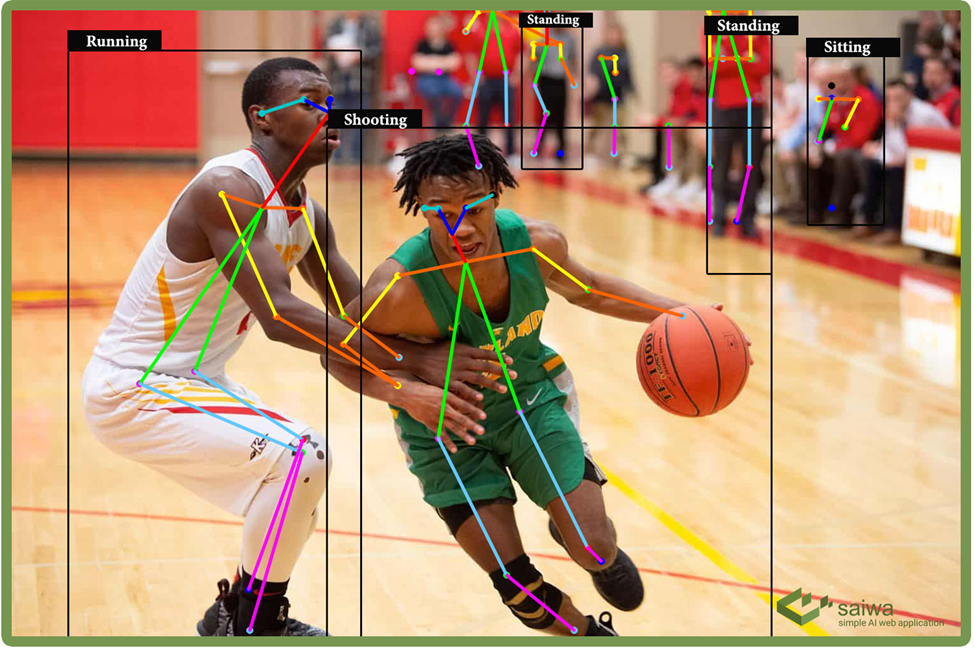
\includegraphics[width=\textwidth]{"images/1_DTaPdSzIw4rMmD-6hO15rQ.png"}
			\end{subfigure}
			\begin{subfigure}[b]{0.4\textwidth}
				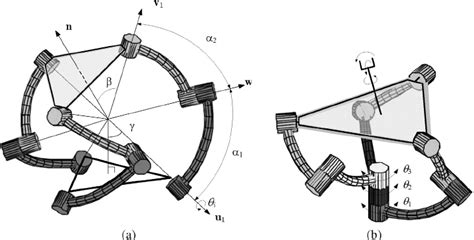
\includegraphics[width=\textwidth]{"images/th-2320009920.jpg"}
			\end{subfigure}
		\end{figure}
	\end{frame}
	\begin{frame}
		\begin{dfn}[3Q3-Problem]\pause
			Sei $K$ ein Körper und seien $X_1$,$X_{2}$ und $X_{3}$ die Unbestimmten unseres Gleichungssystems. Weiter bezeichne $C \in K^{3\times 10}$ die Koeffizientenmatrix. Das Gleichungssystem, welches es zu lösen gilt, lautet dann
			\begin{gather}\label{eqn:3Q3}
				\begin{alignedat}{4}
					c_{1,1}X_{1}^2&+c_{1,2}X_{1}X_{2}+c_{1,3}X_{1}X_{3}+c_{1,4}X_{2}^2+c_{1,5}X_{2}X_{3}\ldots&&&\\&+c_{1,6}X_{3}^2+c_{1,7}X_{1}+c_{1,8}X_{2}+c_{1,9}X_{3}+c_{1,10}=0,\\
					c_{2,1}X_{1}^2&+c_{2,2}X_{1}X_{2}+c_{2,3}X_{1}X_{3}+c_{2,4}X_{2}^2+c_{2,5}X_{2}X_{3}\ldots&&&\\&+c_{2,6}X_{3}^2+c_{2,7}X_{1}+c_{2,8}X_{2}+c_{2,9}X_{3}+c_{2,10}=0,\\
					c_{3,1}X_{1}^2&+c_{3,2}X_{1}X_{2}+c_{3,3}X_{1}X_{3}+c_{3,4}X_{2}^2+c_{3,5}X_{2}X_{3}\ldots&&&\\&+c_{3,6}X_{3}^2+c_{3,7}X_{1}+c_{3,8}X_{2}+c_{3,9}X_{3}+c_{3,10}=0.\\
				\end{alignedat}
			\end{gather}
		\end{dfn}
	\end{frame}
	\begin{frame}
		\frametitle{Geometrie des 3Q3-Problems}
		\begin{itemize}
			\pause
			\item Über $\R$ besitzt das 3Q3-Problem eine anschauliche geometrische Interpretation des Gleichungssystems.
			\pause
			\item Über den reellen Zahlen beschreibt jede der Gleichungen eine Quadrik im Raum.
			\pause
			\item Die Lösungen des 3Q3-Problems sind genau die Punkte, in denen sich alle drei Quadriken gemeinsam schneiden.
		\end{itemize}
	\end{frame}
	\section{Betrachtung in der algebraischen Geometrie}
	\begin{frame}
		\begin{dfn}[Algebraische Menge]\label{def:alg_menge}
			\pause
			Sei $K$ ein Körper und $\tilde{K}$ der zugehörige algebraische Abschluss.
			Eine Teilmenge $V \subset \tilde{K}^n$ zu einem Körper $K$ heißt affine, algebraische Menge, wenn es ein algebraisches Gleichungssystem gibt, so dass $V$ die Lösungsmenge des Systems ist. Das alg. Gleichungssystem nennt man das definierende Gleichungssystem von $V$ und man sagt $V$ sei definiert über $K$.
			Ist $L \subseteq \tilde{K}^{n}$ ein Erweiterungskörper von $K$, so nennt man die Elemente der Menge
			\begin{equation*}
				V_{L} \coloneqq V \cap L^{n}
			\end{equation*}
			die $L$-rationalen Punkte von $V$.
		\end{dfn}
	\end{frame}
	\begin{frame}
		\begin{dfn}[Algebraische Hyperfläche]
			\pause
			Eine über dem Körper $K$ definierte, affine algebraische Hyperfläche ist eine Teilmenge $H \subset \tilde{K}^{n}$ mit der Gestalt
			\begin{equation}
				H = \{\left( \alpha_{1},\dots,\alpha_{n}\right) \in \tilde{K}^{n} \colon f\left(  \alpha_{1},\dots,\alpha_{n}\right) = 0  \} \ , 
			\end{equation}
			wobei $\tilde{K}^{n}$ den algebraischen Abschluss von $K$ bezeichnet und \newline ${f \in K\left[ X_{1},\dots, X_{n}\right] \setminus K}$ gilt. Man nennt $H$ die durch $f$ definierte Hyperfläche und $f$ ein $H$ definierendes Polynom.\\
			Ist $L \subseteq \tilde{K}^{n}$ ein Erweiterungskörper von $K$, so nennt man die Element der Menge
			\begin{equation*}
				H_{L} \coloneqq H \cap L^{n}
			\end{equation*}
			die $L$-rationalen Punkte von $H$.
		\end{dfn}
	\end{frame}
	\begin{frame}
		\begin{dfn}[Ideal]
			\pause
			Eine Teilmenge $I$ eines kommutativen Ringes $R$, welche die Bedingungen
			\begin{enumerate}
				\item $\forall \ i_1,\ i_2 \in I \colon i_1+i_2 \in I$  
				\item $\forall \ r \in R,\ i \in I \colon r \cdot i \in I$	
			\end{enumerate}
			erfüllt, wird als Ideal von $R$ bezeichnet.
		\end{dfn}
	\end{frame}
	\begin{frame}
		\begin{dfn}
			\pause
			Es seien $R$ ein kommutativer Ring und $I$ ein Ideal von $R$ mit $I \neq R$.
			\begin{enumerate}
				\item Wir nennen $I$ \textbf{maximal}, wenn es kein Ideal $J$ gibt mit $I \subsetneqq J \subsetneqq R$.
				\item Wir nennen $I$ \textbf{prim}, wenn aus $a\cdot b \in I$ stets $a \in I$ oder $b \in I$ folgt.
				\item Wir nennen $I$ \textbf{primär}, wenn aus $a\cdot b \in I$ mit $a \not\in I$ folgt, dass es ein $n \in \N$ gibt mit $b^n \in I$.
				\item $\text{Rad}(I) \coloneqq \sqrt{I} \coloneqq \{x \in R \ \left| \  \exists \, n \in \N \colon x^n \in I\right.\}$ ist ein Ideal von $R$ und wird als Radikal von $I$ bezeichnet.
			\end{enumerate}
		\end{dfn}
	\end{frame}
	\begin{frame}
		\begin{proposition}\label{prop:bezout}
			\pause
			Es seien $K$ ein algebraisch abgeschlossener Körper und $f_1,\ldots,f_m$ $\in$ \newline $K[X_1,\ldots,X_n]$ Polynome der Grade $d_1,\ldots,d_m \in \N$. Besitzt das algebraische Gleichungssystem
			\begin{equation*}
				\begin{alignedat}{5}
					&f_{1}&\left(X_{1}, \ldots, X_{n} \right)& \ &=\ &0\\
					&f_{2}&\left(X_{1}, \ldots, X_{n} \right)& \ &=\ &0\\
					&&&  \vdots& &\\
					&f_{m}&\left(X_{1}, \ldots, X_{n} \right)& \ &=\ &0
				\end{alignedat}
			\end{equation*}
			endlich viele Lösungen, so ist deren Anzahl höchstens gleich $d_1 \cdot \ldots \cdot d_m$.
		\end{proposition}
	\end{frame}
	\begin{frame}
		\pause
		Es sei $J \coloneqq (f_1,\ldots,f_m)$ das von den Polynomen aus Satz \ref{prop:bezout} erzeugte Ideal von $K[X_1,\ldots,X_n]$.
		Nach dem Hilbert'schen Nullstellensatz liefert die Zuordnung
		\begin{equation*}
			(a_1,\ldots,a_n) \in K^n \mapsto (X_1 - a_1, \ldots,X_n - a_n)
		\end{equation*}
		eine bijektive Abbildung der Lösungen eines Polynomgleichungssystems auf diejenigen maximalen Ideale von $K[X_1,\ldots,X_n]$, die $J$ enthalten. Es genügt also die Kardinalität der Menge
		\begin{equation*}
			\{p \subset K[X_1,\ldots,X_n] \colon J \subseteq p, p \ \text{maximal}\}
		\end{equation*}
		zu bestimmen.
	\end{frame}
	\begin{frame}
		\pause
		Zwischen Prim-, Primäridealen und maximalen Idealen bestehen die folgenden Beziehungen.
		\begin{lemma}\label{cor:prim_max}
			\pause
			Es sei $I$ ein primäres Ideal eines kommutativen Ringes $R$, dann ist $\sqrt{I}$ prim.
		\end{lemma}
		\begin{lemma}
			\pause
			Sei $q$ ein primäres Ideal mit $J \subseteq q$, so ist $\sqrt{q}$ ein maximales Ideal.
		\end{lemma}
	\end{frame}
	\begin{frame}
		\begin{thm}[Lasker-Noether]
			\pause
			Jedes Ideal $I$ eines Polynomrings $K[X_1,\ldots,X_n]$ besitzt eine Darstellung
			\[I = q_1 \cap \ldots \cap q_r\]
			als Schnitt primärer Ideale $q_i$ für die Folgendes gilt:
			\begin{enumerate}
				\item Kein $q_i$ kann weggelassen werden.
				\item Die Primideale $\sqrt{q_1}, \ldots, \sqrt{q_r}$ sind paarweise verschieden.
			\end{enumerate}
			Die Primideale $\sqrt{q_i}$ (aber nicht die Ideale $q_i$) sind dabei durch $I$ eindeutig bestimmt. Die Ideale $q_i$ heißen Primärkomponenten von $I$.
		\end{thm}
	\end{frame}
	\begin{frame}
		\begin{dfn}
			\pause
			Eine Primärkomponente $q_i$ eines Ideal $I \subset K[X_1,\ldots,X_n]$ heißt isoliert, falls das Primideal $\sqrt{q_i}$ in keinem der Primideale $\sqrt{q_j}$ enthalten ist.
		\end{dfn}
		\begin{dfn}
			\pause
			Die Höhe (in Masser \cite{masser1983fields} mit Rang bezeichnet) eines Primideals $p$ von $K[X_1,\ldots,X_n]$ ist die Länge $l$ der längsten Kette \[0=p_0 \subset p_1 \subset \ldots \subset p_l = p\] von Primidealen $p_i$. Es gilt $l \leq n$ mit Gleichheit genau dann, wenn $p$ ein maximales Ideal ist.
		\end{dfn}
	\end{frame}
	\begin{frame}
		\begin{lemma}\label{cor:gls_prim_max}
			\pause
			Im Fall des Ideals $J$ zum Polynomgleichungssystem aus Satz \ref{prop:bezout} sind alle
			Primärkomponenten isoliert, denn nach Korollar \ref{cor:prim_max} sind  die Primideale $\sqrt{q_i}$ alle maximal. Die Menge $\{\sqrt{q_1},\ldots,\sqrt{q_r}\}$ besteht sogar aus allen maximalen Idealen, welche $J$ enthalten.
		\end{lemma}
	\end{frame}
	\begin{frame}
		\begin{dfn}
			\pause
			Die Länge $l(q)$ eines Primärideals $q \subset K[X_1,\ldots,X_n]$ ist wie folgt definiert: Man bildet den Bruchring \[R_p \coloneqq \left\lbrace \frac{z}{n} \colon z \in  K[X_1,\ldots,X_n], n \in  K[X_1,\ldots,X_n] \setminus q \right\rbrace.\]
			Für jedes Ideal $J \subset K[X_1,\ldots,X_n], J \subseteq p$, ist die Menge \[JR_p \coloneqq \{a\cdot r \colon a \in J, r \in R_p\}\]
			ein Ideal von $R_p$.\\
			$pR_p$ ist ein maximales Ideal von $R_p$ und die Länge der längsten Kette \[J_0 \coloneqq qR_p \subset J_1 \subset \ldots \subset J_l \coloneqq pR_p\] ist die zu definierende Länge $l(q)$.
		\end{dfn}
	\end{frame}
	\begin{frame}
		\begin{dfn}
			Ist $J \subseteq K[X_1,\ldots,X_n]$ ein Ideal, das eine Darstellung $J = q_1 \cap \ldots \cap q_r$ als Schnitt von isolierten Primäridealen $q_i$ besitzt, so ist die Länge von $J$ definiert als \[l(J) \coloneqq \sum_{i=1}^{r} l(q_i).\]
		\end{dfn}
	\end{frame}
	\begin{frame}
		\begin{proof}[Beweis zu Satz \ref{prop:bezout}]
			\pause
			Es sei \[I \coloneqq (f_1, \ldots, f_m) = q_1 \cap \ldots \cap q_r\] eine Darstellung von $I$ nach dem Satz von Lasker-Noether. Nach sind alle Primärkomponenten $q_i$ isoliert, womit die Länge von $I$ definiert ist. Nach Definition gilt \[l(I) = \sum_{i=1}^{r} l(q_i)\geq r\] und nach dem Hilbert'schen Nullstellensatz und \ref{cor:gls_prim_max} ist $r$ die Anzahl verschiedener Lösungen der algebraischen Gleichungssystems. Man wendet nun das Korollar für den Fall $s=n$ an, da die Primideale $\sqrt{q_i}$ maximal sind, also den Rang $n$ besitzen. Es ist $t \leq m$ und damit \[M_t(d_1, \ldots, d_m) \leq d_1 \cdot \ldots \cdot d_m,\] woraus die Aussage des Satzes folgt.
		\end{proof}
	\end{frame}
	\section{Der E3Q3-Algorithmus}
	\begin{frame}
		\frametitle{Der E3Q3-Algorithmus}
		\pause
		Es liege nun das 3Q3-Problem in der Form
		\begin{equation*}
			\small
			\begin{pmatrix}
				c_{1,1}&c_{1,2}&\ldots&c_{1,10}\\
				c_{2,1}&c_{2,2}&\ldots&c_{2,10}\\
				c_{3,1}&c_{3,2}&\ldots&c_{3,10}\\
			\end{pmatrix} \cdot
			\begin{pmatrix}
				X_{1}^{2},X_{1}X_{2},X_{1}X_{3},X_{2}^{2},X_{2}X_{3},X_{3}^{2},X_{1},X_{2},X_{3},1
			\end{pmatrix}^\top =  \begin{pmatrix}
				0\\0\\0
			\end{pmatrix}
		\end{equation*}
		vor.\\
	\end{frame}
	\begin{frame}
		\begin{equation}\label{eqn:E3Q3}
			\begin{alignedat}{6}
				&p_{11}^{\left[1\right] }\left(X_{1}\right)X_{2}+
				&p_{12}^{\left[1\right] }\left(X_{1}\right)X_{3}+
				&p_{13}^{\left[2\right] }\left(X_{1}\right)+
				&c_{14}X_{2}^2+&c_{15}X_{2}X_{3}+&c_{16}X_{3}^2=0,\\
				&p_{21}^{\left[1\right] }\left(X_{1}\right)X_{2}+
				&p_{22}^{\left[1\right] }\left(X_{1}\right)X_{3}+
				&p_{23}^{\left[2\right] }\left(X_{1}\right)+
				&c_{24}X_{2}^2+&c_{25}X_{2}X_{3}+&c_{26}X_{3}^2=0,\\
				&p_{31}^{\left[1\right] }\left(X_{1}\right)X_{2}+
				&p_{32}^{\left[1\right] }\left(X_{1}\right)X_{3}+
				&p_{33}^{\left[2\right] }\left(X_{1}\right)+
				&c_{34}X_{2}^2+&c_{35}X_{2}X_{3}+&c_{36}X_{3}^2=0,
			\end{alignedat}
		\end{equation}
		wobei $c_{ij} \in K$ und $p_{ij}^{\left[\cdot \right] } \in K\left[ X_{1}\right]$ gilt und der obere Index $\left[\cdot \right]$ den Maximalgrad des Polynoms darstellt.
	\end{frame}
	\subsection*{Auswahl und Auflösen der Gruppen}
	\begin{frame}
		\begin{equation}\label{eqn:E3Q3}
			\begin{alignedat}{6}
				&p_{11}^{\left[1\right] }\left(X_{1}\right)\textcolor{blue}{X_{2}}+
				&p_{12}^{\left[1\right] }\left(X_{1}\right)\textcolor{blue}{X_{3}}+
				&p_{13}^{\left[2\right] }\left(X_{1}\right)\textcolor{blue}{1}+
				&c_{14}\textcolor{red}{X_{2}^2}+&c_{15}\textcolor{red}{X_{2}X_{3}}+&c_{16}\textcolor{red}{X_{3}^2}=0,\\
				&p_{21}^{\left[1\right] }\left(X_{1}\right)\textcolor{blue}{X_{2}}+
				&p_{22}^{\left[1\right] }\left(X_{1}\right)\textcolor{blue}{X_{3}}+
				&p_{23}^{\left[2\right] }\left(X_{1}\right)\textcolor{blue}{1}+
				&c_{24}\textcolor{red}{X_{2}}^2+&c_{25}\textcolor{red}{X_{2}X_{3}}+&c_{26}\textcolor{red}{X_{3}^2}=0,\\
				&p_{31}^{\left[1\right] }\left(X_{1}\right)\textcolor{blue}{X_{2}}+
				&p_{32}^{\left[1\right] }\left(X_{1}\right)\textcolor{blue}{X_{3}}+
				&p_{33}^{\left[2\right] }\left(X_{1}\right)\textcolor{blue}{1}+
				&c_{34}\textcolor{red}{X_{2}^2}+&c_{35}\textcolor{red}{X_{2}X_{3}}+&c_{36}\textcolor{red}{X_{3}^2}=0,
			\end{alignedat}
		\end{equation}
		wobei $c_{ij} \in K$ und $p_{ij}^{\left[\cdot \right] } \in K\left[ X_{1}\right]$ gilt und der obere Index $\left[\cdot \right]$ den Maximalgrad des Polynoms darstellt.
	\end{frame}
	\begin{frame}
		\begin{equation}\label{eqn:E3Q3_sep}
			- \ 
			C \
			\begin{pmatrix}
				X_{2}^2\\X_{2}X_{3}\\X_{3}^2
			\end{pmatrix} 
			=
			P \
			\begin{pmatrix}
				X_{2}\\X_{3}\\1
			\end{pmatrix},
		\end{equation}
		mit den Matrizen
		\begin{equation*}
			C = \begin{pmatrix}
				c_{14}&c_{15}&c_{16}\\
				c_{24}&c_{25}&c_{26}\\
				c_{34}&c_{35}&c_{36}\\
			\end{pmatrix} \in K^{3 \times 3}
		\end{equation*}
		und
		\begin{equation*}
			P = \begin{pmatrix}p_{11}\left(X_{1}\right)&p_{12}\left(X_{1}\right)&p_{13}\left(X_{1}\right)\\
				p_{21}\left(X_{1}\right)&p_{22}\left(X_{1}\right)&p_{23}\left(X_{1}\right)\\
				p_{31}\left(X_{1}\right)&p_{32}\left(X_{1}\right)&p_{33}\left(X_{1}\right)\\
			\end{pmatrix} \in K[X_1]^{3 \times 3}
		\end{equation*}
	\end{frame}
	\begin{frame}
		Wenn die Matrix $C$ invertierbar ist erhalten wir das System\\
		\begin{equation}\label{eqn:E3Q3_inv}
			\small
			\begin{pmatrix}
				X_{2}^2\\X_{2}X_{3}\\X_{3}^2
			\end{pmatrix} 
			=
			C^{-1} \cdot P(X_{1})
			\begin{pmatrix}
				X_{2}\\X_{3}\\1
			\end{pmatrix}
			=
			\begin{pmatrix}
				p'_{11}\left(X_{1}\right)&p'_{12}\left(X_{1}\right)&p'_{13}\left(X_{1}\right)\\
				p'_{21}\left(X_{1}\right)&p'_{22}\left(X_{1}\right)&p'_{23}\left(X_{1}\right)\\
				p'_{31}\left(X_{1}\right)&p'_{32}\left(X_{1}\right)&p'_{33}\left(X_{1}\right)\\
			\end{pmatrix}
			\begin{pmatrix}
				X_{2}\\X_{3}\\1
			\end{pmatrix}
			.
		\end{equation}
		~\\
		Mithilfe von Gleichung \eqref{eqn:E3Q3_inv} lassen sich die quadratischen Monome $X_{2}^2$, $X_{3}^2$ und $X_{2}X_{3}$ durch Linearkombinationen aus den Monomen $X_{2}$,$X_{3}$,$1$ mit Koeffizienten in $K\left[X_{1}\right] $ schreiben.
	\end{frame}
	\subsection*{Substitution der Identitäten}
	\begin{frame}
		\begin{equation}
			\begin{alignedat}{-1}
				&\left(X_{2}^2\right) &X_{3}\ & &=& &\Bigl(X_{2}X_{3} \Bigr)&  X_{2},\\
				&\left(X_{3}^2\right) &X_{2}\ & &=& &\Bigl(X_{2}X_{3} \Bigr)&  X_{3},\\
				&\left(X_{2}^2\right) &\left( X_{3}^2\right)&  &=& &\Bigl(X_{2}X_{3} \Bigr)&  \Bigl(X_{2}X_{3} \Bigr).
			\end{alignedat}
		\end{equation}
	\end{frame}
	\begin{frame}
		Da die Substitutionen für $\textcolor{red}{X_{2}^2}$, $\textcolor{red}{X_{3}^2}$ und $\textcolor{red}{X_{2}X_{3}}$ aus Linearkombinationen in \textcolor{blue}{$X_{2}$} und \textcolor{blue}{$X_{3}$} bestehen, erhalten wir nach der ersten Substitution das Gleichungssystem
		\begin{equation}
			\begin{alignedat}{1}
				p'_{11}\textcolor{red}{X_{2}X_{3}}+p'_{12}\textcolor{red}{X_{3}^2}+p'_{13}\textcolor{blue}{X_{3}}&=p'_{21}\textcolor{red}{X_{2}^2}+p'_{22}\textcolor{red}{X_{2}X_{3}}+p'_{23}\textcolor{blue}{X_{2}},\\
				p'_{31}\textcolor{red}{X_{2}^2}+p'_{32}\textcolor{red}{X_{2}X_{3}}+p'_{33}\textcolor{blue}{X_{2}}&=p'_{21}\textcolor{red}{X_{2}X_{3}}+p'_{22}\textcolor{red}{X_{3}^2}+p'_{23}\textcolor{blue}{X_{3}},\\
				\left(p'_{21}X_{2}+p'_{22}X_{3}+p'_{23}\right)^2&=\left( p'_{11}X_{2}+p'_{12}X_{3}+p'_{13}\right)\\ & \quad \cdot \left( p'_{31}X_{2}+p'_{32}X_{3}+p'_{33}\right),
			\end{alignedat}
		\end{equation}
		wobei die $p'_{ij} \in K[X_{1}]$ die Polynome aus Gleichung \eqref{eqn:E3Q3_inv} sind.
	\end{frame}
	\begin{frame}
		Nach nochmaliger Substitution ergibt sich das lineare Gleichungssystem
		\begin{equation}\label{eqn:E3Q3_M_eq}
			\begin{pmatrix}[1.5]
				m_{11}^{\left[ 2\right]}\left( X_{1}\right) & m_{12}^{\left[ 2\right]}\left( X_{1}\right) & m_{13}^{\left[ 3\right]}\left( X_{1}\right) \\
				m_{21}^{\left[ 2\right]}\left( X_{1}\right) & m_{22}^{\left[ 2\right]}\left( X_{1}\right) & m_{23}^{\left[ 3\right]}\left( X_{1}\right) \\
				m_{31}^{\left[ 2\right]}\left( X_{1}\right) & m_{32}^{\left[ 2\right]}\left( X_{1}\right) & m_{33}^{\left[ 3\right]}\left( X_{1}\right) \\
			\end{pmatrix}
			\begin{pmatrix}[1.5]
				X_{2}\\
				X_{3}\\
				1
			\end{pmatrix}
			= M\left( X_{1}\right) \ \begin{pmatrix}[1.5]
				X_{2}\\
				X_{3}\\
				1
			\end{pmatrix}
			=0.
		\end{equation}
		\pause
		Mithilfe linearer Algebra wissen wir:\\
		Das lineare Gleichungsystem besitzt Lösungen $x_2$ und $x_3$ genau dann, wenn $M\left( X_{1}\right)$ als polynomiale Matrix über $K[X_{1}]^{3 \times 3}$ regulär ist und \begin{equation}\label{eqn:det_zero}
			\det\left(M\left( X_{1}\right)  \right) = 0
		\end{equation}
		erfüllt ist.
	\end{frame}
	\subsection*{Lösen der Gleichungen}
	\begin{frame}
		\begin{itemize}
			\item Aus unserem Theorem erwarten wir bis zu $2^3=8$ Lösungen.
		\pause
		\item Da $\det\left(M\left( X_{1}\right)  \right)$ ein Polynom mit höchstens Grad 8 ist, erhalten wir bis zu 8 Lösungskandidaten $\tilde{x}_1$.
		\pause
		\item Einsetzen ergibt das lineare Gleichungssystem
		\begin{equation}\label{eqn:M_lsg}
			\begin{pmatrix}
				\tilde{m}_{11} & \tilde{m}_{12}\\
				\tilde{m}_{21} & \tilde{m}_{22}\\
				\tilde{m}_{31} & \tilde{m}_{32}\\
			\end{pmatrix}
			\begin{pmatrix}[1.5]
				X_{2}\\
				X_{3}
			\end{pmatrix}
			= -\ \begin{pmatrix}
				\tilde{m}_{13}\\
				\tilde{m}_{23}\\
				\tilde{m}_{33}
			\end{pmatrix},
		\end{equation}
		wobei $r \coloneqq \text{rank}\left(\tilde{M}\right) \leq 2$ gilt.

		\item Durch die möglichen normierten Zeilenstufenformen ergeben sich drei Fälle, welche Lösungen $\tilde{x}_2$ und $\tilde{x}_3$ liefern.
				\end{itemize}
	\end{frame}
	\subsection*{Zusammenfassung}
	\begin{frame}
		\frametitle{Schritte des E3Q3 Algorithmus}
		\begin{enumerate}
			\pause
			\item \glqq Verstauen\grqq~einer Unbestimmten im Koeffizientenbereich\pause
			\item Aufteilen der verbleibenden Monome in zwei Gruppen\pause
			\item Auflösen nach den Monomen in einer Gruppe\pause
			\item Substituierung der Monome mittels Identitäten\pause
			\item Lösen des resultierenden Gleichungssystems
		\end{enumerate}
	\end{frame}
	\subsection*{Beispiele}
	\begin{frame}
		\begin{exm}
			Gegeben sei das Gleichungssystem	
			\begin{equation*}\label{eqn:example5}
				\begin{alignedat}{-1}
					x^2+3\,y^2+y\,z+z^2-5&=0,\\
					3\,x^2+2\,y^2+2\,y\,z+z^2-5&=0,\\
					2\,x^2+y^2-y\,z+2\,z^2-5&=0
				\end{alignedat}
			\end{equation*}
			über $\R$.
		\end{exm}
	\end{frame}
	\begin{frame}
		\begin{exm}
			Gegeben sei das Gleichungssystem
			\begin{equation*}
				\small
				\begin{alignedat}{-1}
					29236\,x^2+5262\,x+13670\,y+29511\,z+52080\,y\,z-5044&=0,\\ -6089\,x+6437\,y-3619\,z+9520\,x\,z+16456\,y\,z+36592\,z^2+20861&=0,\\ 40362\,y^2+18928\,y+17093\,x+1294\,z+29534&=0
				\end{alignedat}
			\end{equation*}
			über $\F{69427}$.
		\end{exm}
	\end{frame}
	\section{Erweiterung auf kubische Flächen}
	\begin{frame}
		\frametitle{Das mC3 Problem}
		\begin{dfn}[mC3 Problem]
			Sei $K$ ein Körper und seien $X_1$,$X_{2}$ und $X_{3}$ die Unbestimmten unseres Gleichungssystems. Weiter seien $m \in \N$ und $C \in K^{m\times 20}$ bezeichne die Koeffizientenmatrix. Das Gleichungssystem, welches es zu lösen gilt, lautet dann
			\begin{gather}\label{eqn:mC3}
				\tiny
				\begin{alignedat}{5}
					& c_{1} \cdot &v&,
					&=&0\\
					& c_{2} \cdot &v&,
					&=&0\\
					&&\vdots&&&\\
					& c_{m} \cdot &v&
					&=&0,
				\end{alignedat}
			\end{gather}
			wobei $c_{i}$ für die $i$-te Zeile der Matrix $C$ und $v$ für den Monomvektor 
			\begin{equation*}
				\tiny
				v = 	
				\begin{pmatrix}
					X_{1}^3,X_{1}^2X_{2},X_{1}^2X_{3},X_{1}X_{2}^2,X_{1}X_{2}X_{3},X_{1}X_{3}^2,X_{2}^3,X_{3}^3,X_{2}^2X_{3},\ldots \\
					X_{2}X_{3}^2,X_{1}^2,X_{1}X_{2},X_{1}X_{3},X_{2}^2,X_{2}X_{3},X_{3}^2,X_{1},X_{2},X_{3},1
				\end{pmatrix}
				^{\top} \in K[X_1,X_2,X_3]^{20}
			\end{equation*}
			steht.
		\end{dfn}
	\end{frame}
	\subsection*{Aufteilen in zwei Gruppen und Auflösen}
	\begin{frame}
		\frametitle{Aufteilen in zwei Gruppen und Auflösen}
		\begin{itemize}
			\item Nach Verstauen der Unbekannten $X_1$ bleiben die $10$ Monome
			\begin{equation*}
				\lbrace X_2^3,X_2^2X_3,X_2X_3^2,X_3^3,X_2^2,X_2X_3,X_3^2,X_2,X_3,1 \rbrace
			\end{equation*}
			\item Wir teilen die Monome in die Gruppen
			$G_1 \coloneqq \{\mu_1,\ldots,\mu_n\}$ und $G_2 \coloneqq \{\eta_1,\ldots,\eta_{10-n}\}$ ein.
		\end{itemize}
		
	\end{frame}
		\begin{frame}
		\frametitle{Aufteilen in zwei Gruppen und Auflösen}
		\begin{itemize}
			\item Das aufgeteilte Gleichungssystem ergibt sich dann als
			\begin{equation*}
				-A \cdot \left(\mu_1,\ldots,\mu_n\right)^{\top} = P \cdot \left(\eta_1,\ldots,\eta_{o}\right)^{\top},
			\end{equation*}
			mit den Matrizen $A \in K[X_1]^{m \times n}$ und $P \in K[X_1]^{m \times (10-n)}$.

				\item Damit wir auflösen können, muss $A$ invertierbar sein und somit offensichtlich $m=n$ gelten.
		\end{itemize}
	\end{frame}
	\begin{frame}
		\frametitle{Aufteilen in zwei Gruppen und Auflösen}
		\begin{itemize}
			\item Das aufgeteilte Gleichungssystem ergibt sich dann als
			\begin{equation*}
				-A \cdot \left(\mu_1,\ldots,\mu_n\right)^{\top} = P \cdot \left(\eta_1,\ldots,\eta_{o}\right)^{\top},
			\end{equation*}
			mit den Matrizen $A \in K[X_1]^{m \times n}$ und $P \in K[X_1]^{m \times (10-n)}$.
				\item Damit wir auflösen können, muss $A$ invertierbar sein und somit offensichtlich \textcolor{red}{$m=n$} gelten.
		\end{itemize}
	\end{frame}
	\subsection*{Substituieren in Identitäten}
	\begin{frame}
		\frametitle{Substituieren in Identitäten}
		\begin{itemize}
			\item Wir wollen von unserem isolierten System
			\begin{equation*}\label{eqn:cub_inv_eqs}
				\left(\mu_1,\ldots,\mu_n\right)^{\top} = -A^{-1} P \cdot \left(\eta_1,\ldots,\eta_{10-n}\right)^{\top},
			\end{equation*}
			durch Substitution zu einem Gleichungssystem
			\begin{equation*}
				M(X_1) \cdot \left(\eta_1,\ldots,\eta_{10-n} \right)^{\top} = 0
			\end{equation*}
			gelangen, wobei die Matrix $M(X_1) \in K[X_1]^{(10-n) \times (10-n)}$ ist.
			\item Wir brauchen also $10-n$ Identitäten in den Monomen $\mu_1,\ldots,\mu_n$.
			\item Außerdem dürfen nach der Substitution nur Terme in den Monomen $\left(\mu_1,\ldots,\mu_n,\eta_1,\ldots,\eta_{10-n}\right)$ vorkommen.
		\end{itemize}
	\end{frame}
	\begin{frame}
		\frametitle{Substituieren in Identitäten}
		\begin{itemize}
			\item Wir wollen von unserem isolierten System
			\begin{equation*}\label{eqn:cub_inv_eqs}
				\left(\mu_1,\ldots,\mu_n\right)^{\top} = -A^{-1} P \cdot \left(\eta_1,\ldots,\eta_{10-n}\right)^{\top},
			\end{equation*}
			durch Substitution zu einem Gleichungssystem
			\begin{equation*}
				M(X_1) \cdot \left(\eta_1,\ldots,\eta_{10-n} \right)^{\top} = 0
			\end{equation*}
			gelangen, wobei die Matrix $M(X_1) \in K[X_1]^{(10-n) \times (10-n)}$ ist.
				\item Wir brauchen also \textcolor{red}{$10-n$} Identitäten in den Monomen $\mu_1,\ldots,\mu_n$.
				\item Außerdem dürfen nach der Substitution nur Terme in den Monomen $\left(\mu_1,\ldots,\mu_n,\eta_1,\ldots,\eta_{10-n}\right)$ vorkommen.
		\end{itemize}
		
	\end{frame}
	\subsection*{Lösen des vereinfachten Gleichungssystems}
	\begin{frame}
		\frametitle{Lösen des vereinfachten Gleichungssystems}
		\begin{itemize}
			\item Die Lösungskandidaten $\tilde{x}_1$ erhalten wir aus
			\begin{equation*}
				\det\left(M(X_1)\right)  = 0.
			\end{equation*}
			\item Das resultierende Gleichungssystem
			\begin{equation*}\label{eqn:low_rank_system}
				\tilde{M}\cdot\begin{pmatrix}[1.3]
					\eta_1,\ldots,\eta_{10-n}
				\end{pmatrix}^\top =0,
			\end{equation*}
			muss dann noch individuell gelöst werden.
		\end{itemize}
	\end{frame}
	\begin{frame}
		\frametitle{Weiteres Vorgehen}
		\begin{itemize}
			\item Wir werden nun den Algorithmus für kubische Flächen für verschiedene Aufteilungen zu formulieren
			\pause
			\item Dabei fangen wir aus Symmetriegründen mit $n=5$ Gleichungen und versuchen die Vorgehensweise auf vier und schließlich drei Gleichungen zu übertragen. 
		\end{itemize}
	\end{frame}
	\section{Ein 5C3-Algorithmus}
	\begin{frame}
		\frametitle{5C3-Algorithmus}
		\begin{itemize}
			\item Wir wählen die Gruppen $\{X_{2}^3,X_{3}^3,X_{2}^2X_{3},X_{2}X_{3}^2,X_{2}X_{3}\}$ und $\{X_{2}^2,X_{3}^2,X_{2},X_{3},1\}$.\\ \pause
		
		\item Teilen wir jetzt die Koeffizientenmatrix $C$ auf beide Gruppen auf ergibt sich 
		\begin{equation*}
			-A
			\begin{pmatrix}
				X_{2}^3\\
				X_{2}^2X_{3}\\
				X_{2}X_{3}^2\\
				X_{3}^3\\
				X_{2}X_{3}
			\end{pmatrix}
			=
			\begin{pmatrix}[1.75]
				\vert & \vert & \vert & \vert & \vert \\
				p_{i,1}(X_{1})&p_{i,2}(X_{1})& p_{i,3}(X_{1})& p_{i,4}(X_{1})& p_{i,5}(X_{1})\\
				\vert & \vert & \vert & \vert & \vert
			\end{pmatrix}
			\begin{pmatrix}
				X_{2}^2\\
				X_{3}^2\\
				X_{2}\\
				X_{3}\\
				1
			\end{pmatrix}.
		\end{equation*}
		\end{itemize}
	\end{frame}
	\begin{frame}
		\begin{itemize}
			\item Damit $A$ invertierbar ist muss $c_{i,5}$ = 0 gelten.
			\item Auflösen nach $G1$ ergibt das System
			\begin{equation*}
				\begin{pmatrix}
					X_{2}^3\\
					X_{2}^2X_{3}\\
					X_{2}X_{3}^2\\
					X_{3}^3\\
					X_{2}X_{3}
				\end{pmatrix}
				=
				{\Large \text{P`($X_1$)}} \,
				\begin{pmatrix}
					X_{2}^2\\
					X_{3}^2\\
					X_{2}\\
					X_{3}\\
					1
				\end{pmatrix}.
			\end{equation*}
		\end{itemize}
	\end{frame}
	\begin{frame}
		Wählen wir die $5$ Identitäten
		\begin{gather*}
			\begin{alignedat}{2}
				X_{3} \cdot \left( X_{2}^{3}\right)  &= \left( X_{2}^{2}X_{3}\right) \cdot& X_{2},\\
				X_{3}\cdot \left(X_{2}^{2}X_{3}\right) &= \left(X_{2}X_{3}^{2}\right) \cdot& X_{2},\\
				X_{2}\cdot\left( X_{3}^{3}\right) &= \left(X_{2}X_{3}^{2}\right) \cdot& X_{3},\\
				\left(X_{2}^{2}X_{3}\right)  &= \Bigl(X_{2}X_{3}\Bigr) \cdot& X_{2},\\
				\left(X_{2}X_{3}^{2}\right)  &= \Bigl(X_{2}X_{3}\Bigr) \cdot& X_{3},\\
			\end{alignedat}
		\end{gather*}
		so erfüllen diese die Voraussetzungen für eine erfolgreiche Substitution.
	\end{frame}
	\begin{frame}
		\begin{itemize}
			\item Aus dem resultierenden System
		\begin{equation*}
			M(X_{1})\cdot\begin{pmatrix}[1.3]
				X_{2}^2,
				X_{3}^2,
				X_{2},
				X_{3},
				1
			\end{pmatrix}^\top=0
		\end{equation*}
		erhalten wir über die Determinante von $M(X_{1})$ Lösungskandidaten.
		\item Da dies kein lineares Gleichungssystem ist, lösen wir erst das lineare System
		\begin{equation*}\label{eqn:low_rank_system_ind}
			\tilde{M} \cdot\begin{pmatrix}
				t,
				u,
				v,
				w,
				1
			\end{pmatrix}^\top
			=0.
		\end{equation*}.
		\item Die Lösung dieses Systems ist ein $(4-r)$-dimensionaler affiner Unterraum, der Gestalt ${v_0 + U \subset K^5}$.
		\item Unsere Lösungen sind dann die Elemente des Schnitts \begin{equation*}
			v_0 + U \bigcap \{(v^2,w^2,v,w,1) : v,w \in K\}
		\end{equation*}
		\end{itemize}
	\end{frame}
	\subsection*{Beispiele}
	\begin{frame}
		\frametitle{}
		\begin{exm}
			Für das Gleichungssystem
		\begin{equation*}\label{eqn:example5C3_1}
			\scriptsize
			\begin{alignedat}{1}
				x^3-3\,x^2\,y-2\,x^2\,z+2\,x^2+6\,x\,y+2\,x\,z-x-y^3+4\,y^2\,z-y^2&\ldots\\
				-y\,z^2-4\,y\,z-5\,y-2\,z^3+5\,z^2+2\,z-2&=0,\\ x^3+2\,x^2\,y-x^2\,z-4\,x^2-3\,x\,y^2+2\,x\,y-x\,z^2+4\,x\,z&\ldots\\
				+2\,x+y^2\,z+3\,y^2-2\,y\,z^2+4\,y\,z-8\,y+2\,z^3-5\,z^2+2\,z+1&=0,\\ -2\,x^3+2\,x^2\,y+x^2\,z+x^2-4\,x\,y^2+2\,x\,y+2\,x\,z^2-8\,x\,z&\ldots\\
				+9\,x-5\,y^3+22\,y^2+2\,y\,z^2-6\,y\,z-20\,y+2\,z^3-8\,z^2+13\,z-3&=0,\\ -2\,x^3+2\,x^2\,y-2\,x^2\,z+6\,x^2-x\,y^2-2\,x\,y+2\,x\,z^2+x\,z&\ldots\\
				-4\,x+2\,y^3-2\,y^2\,z-4\,y^2-2\,y\,z^2+9\,y\,z-4\,y+2\,z^3-5\,z^2-5\,z+9&=0,\\ -2\,x^2\,y-2\,x^2-x\,y^2+6\,x\,y+x\,z&\ldots\\
				+3\,x-3\,y^3+6\,y^2+4\,y\,z^2-8\,y\,z+2\,y-2\,z^2+3\,z-7&=0
			\end{alignedat}
		\end{equation*}
		über $\R$.
		\end{exm}
	\end{frame}
	\begin{frame}
		\begin{figure}[H]
			\label{img:example10}
			\centering
			\begin{subfigure}[b]{0.45\textwidth}
				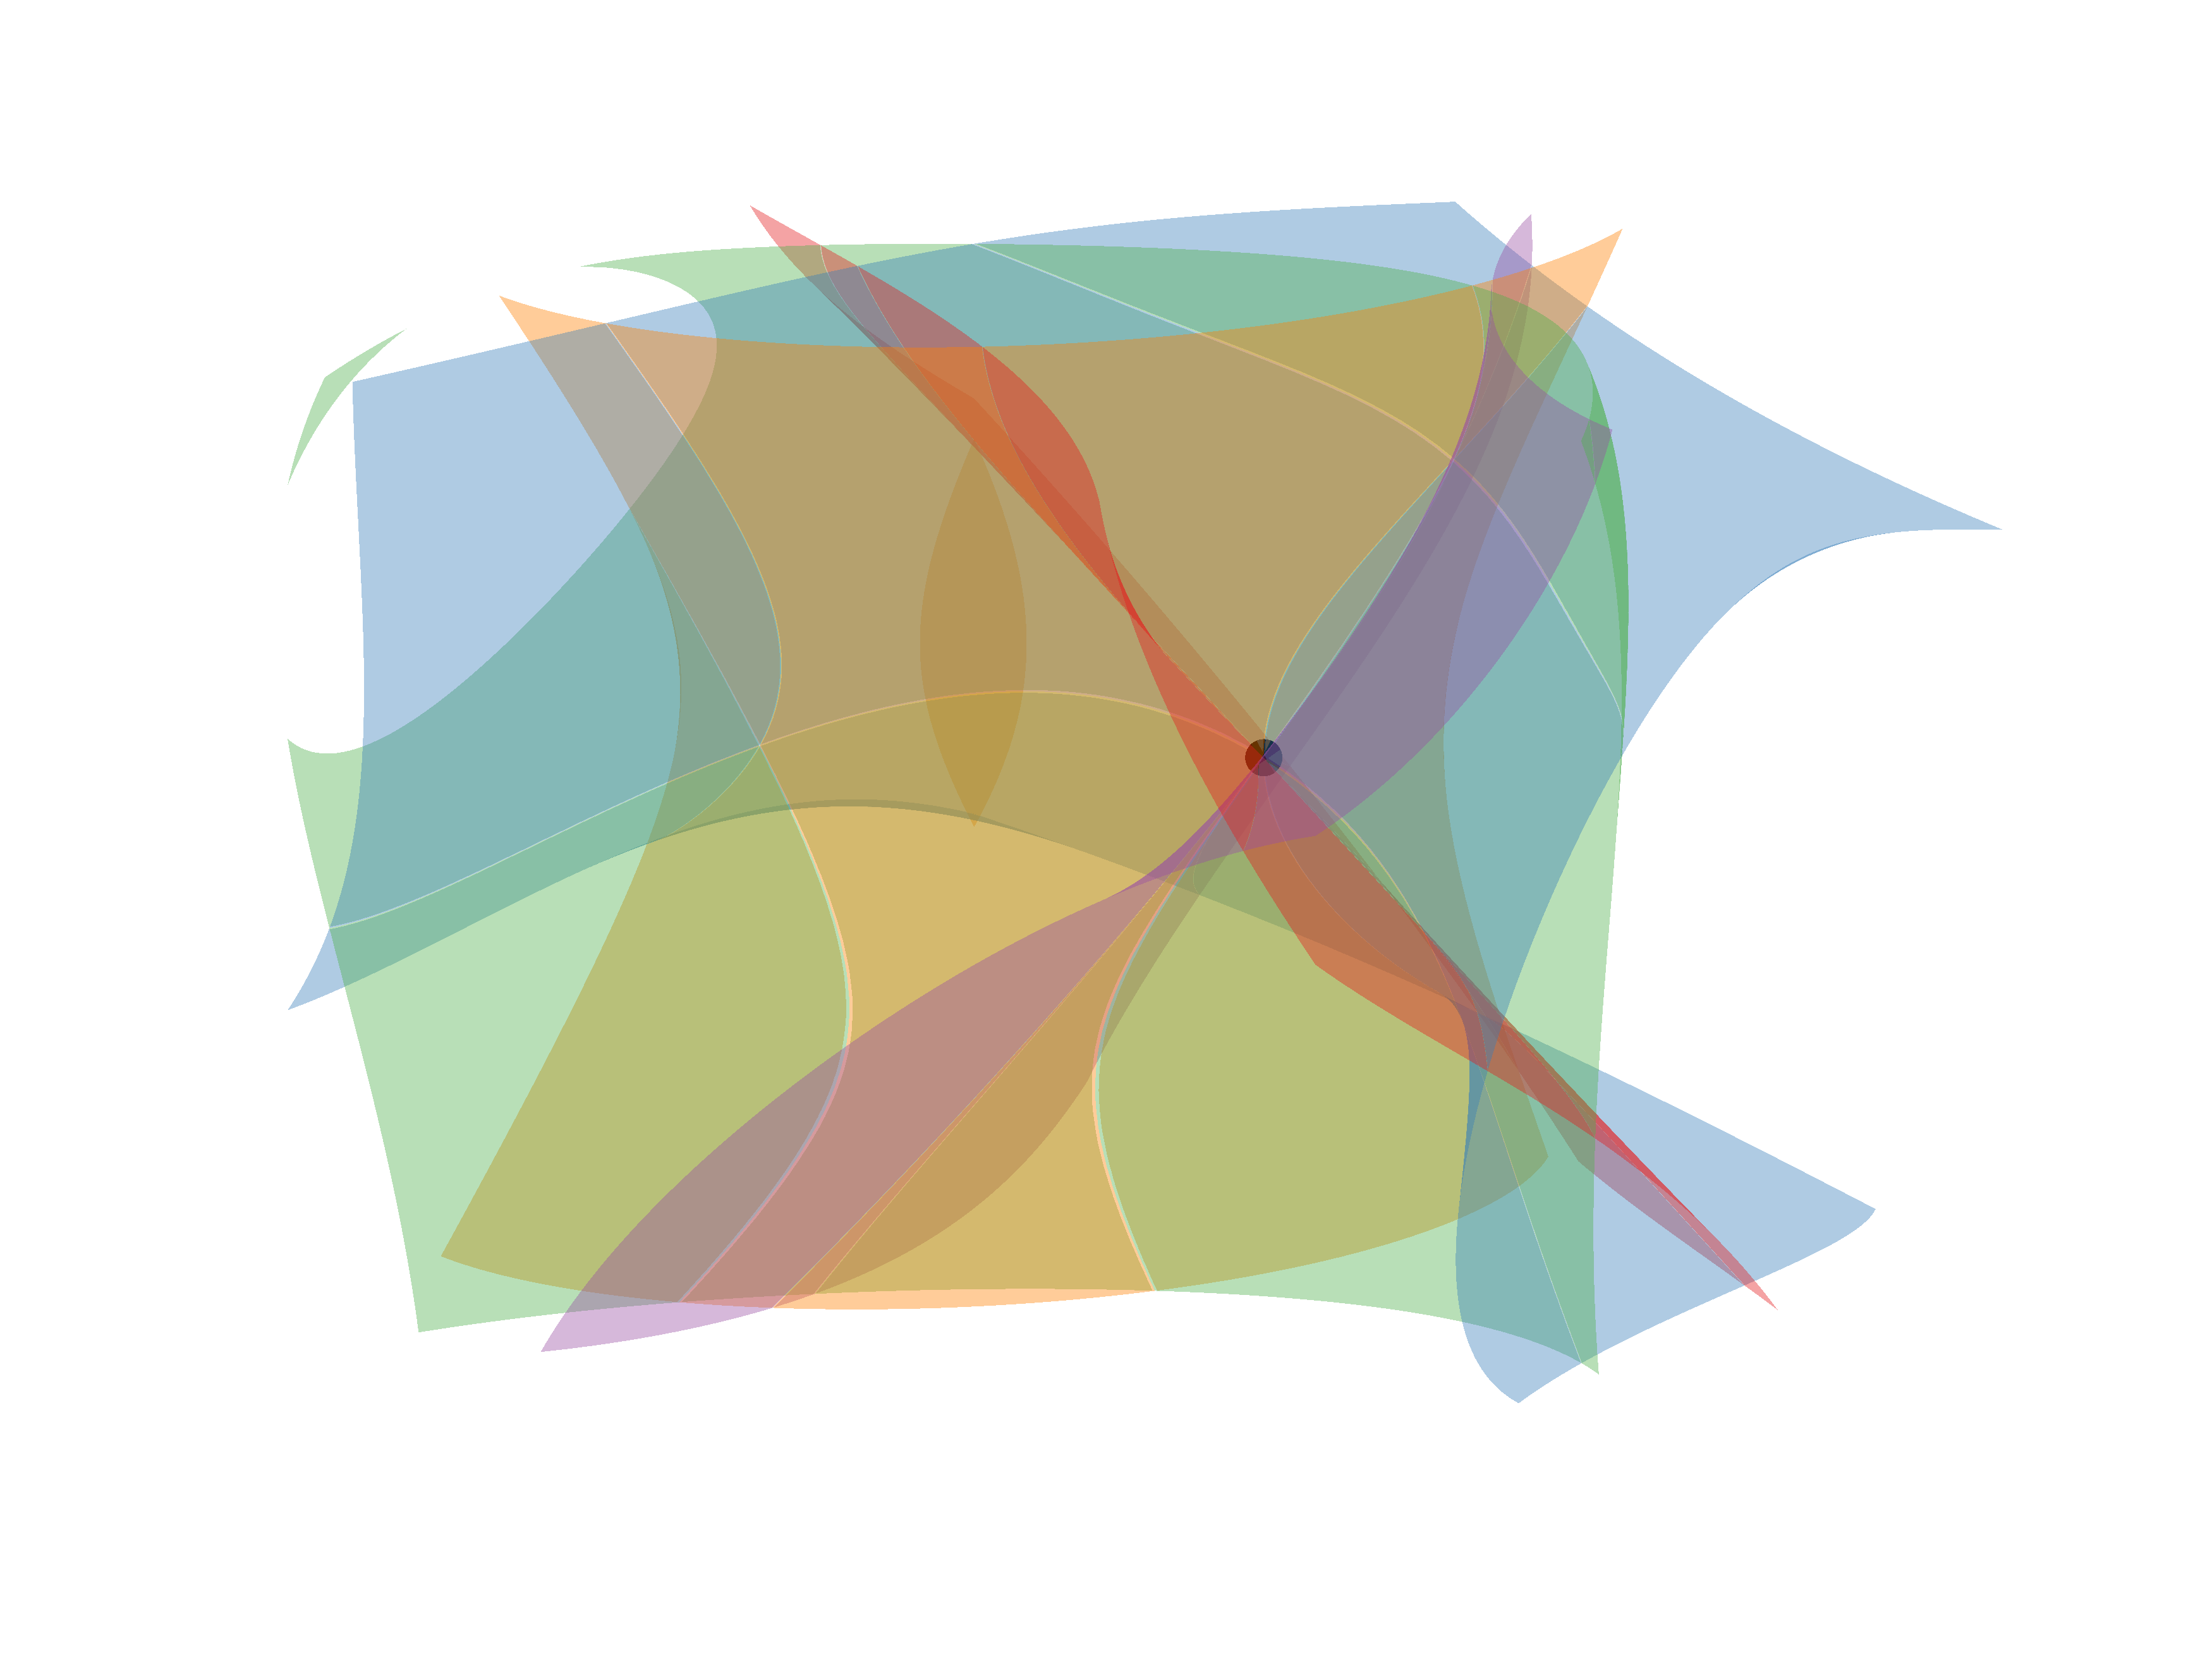
\includegraphics[width=\textwidth]{"images/e5c3_example1.png"}
			\end{subfigure}
			\begin{subfigure}[b]{0.45\textwidth}
				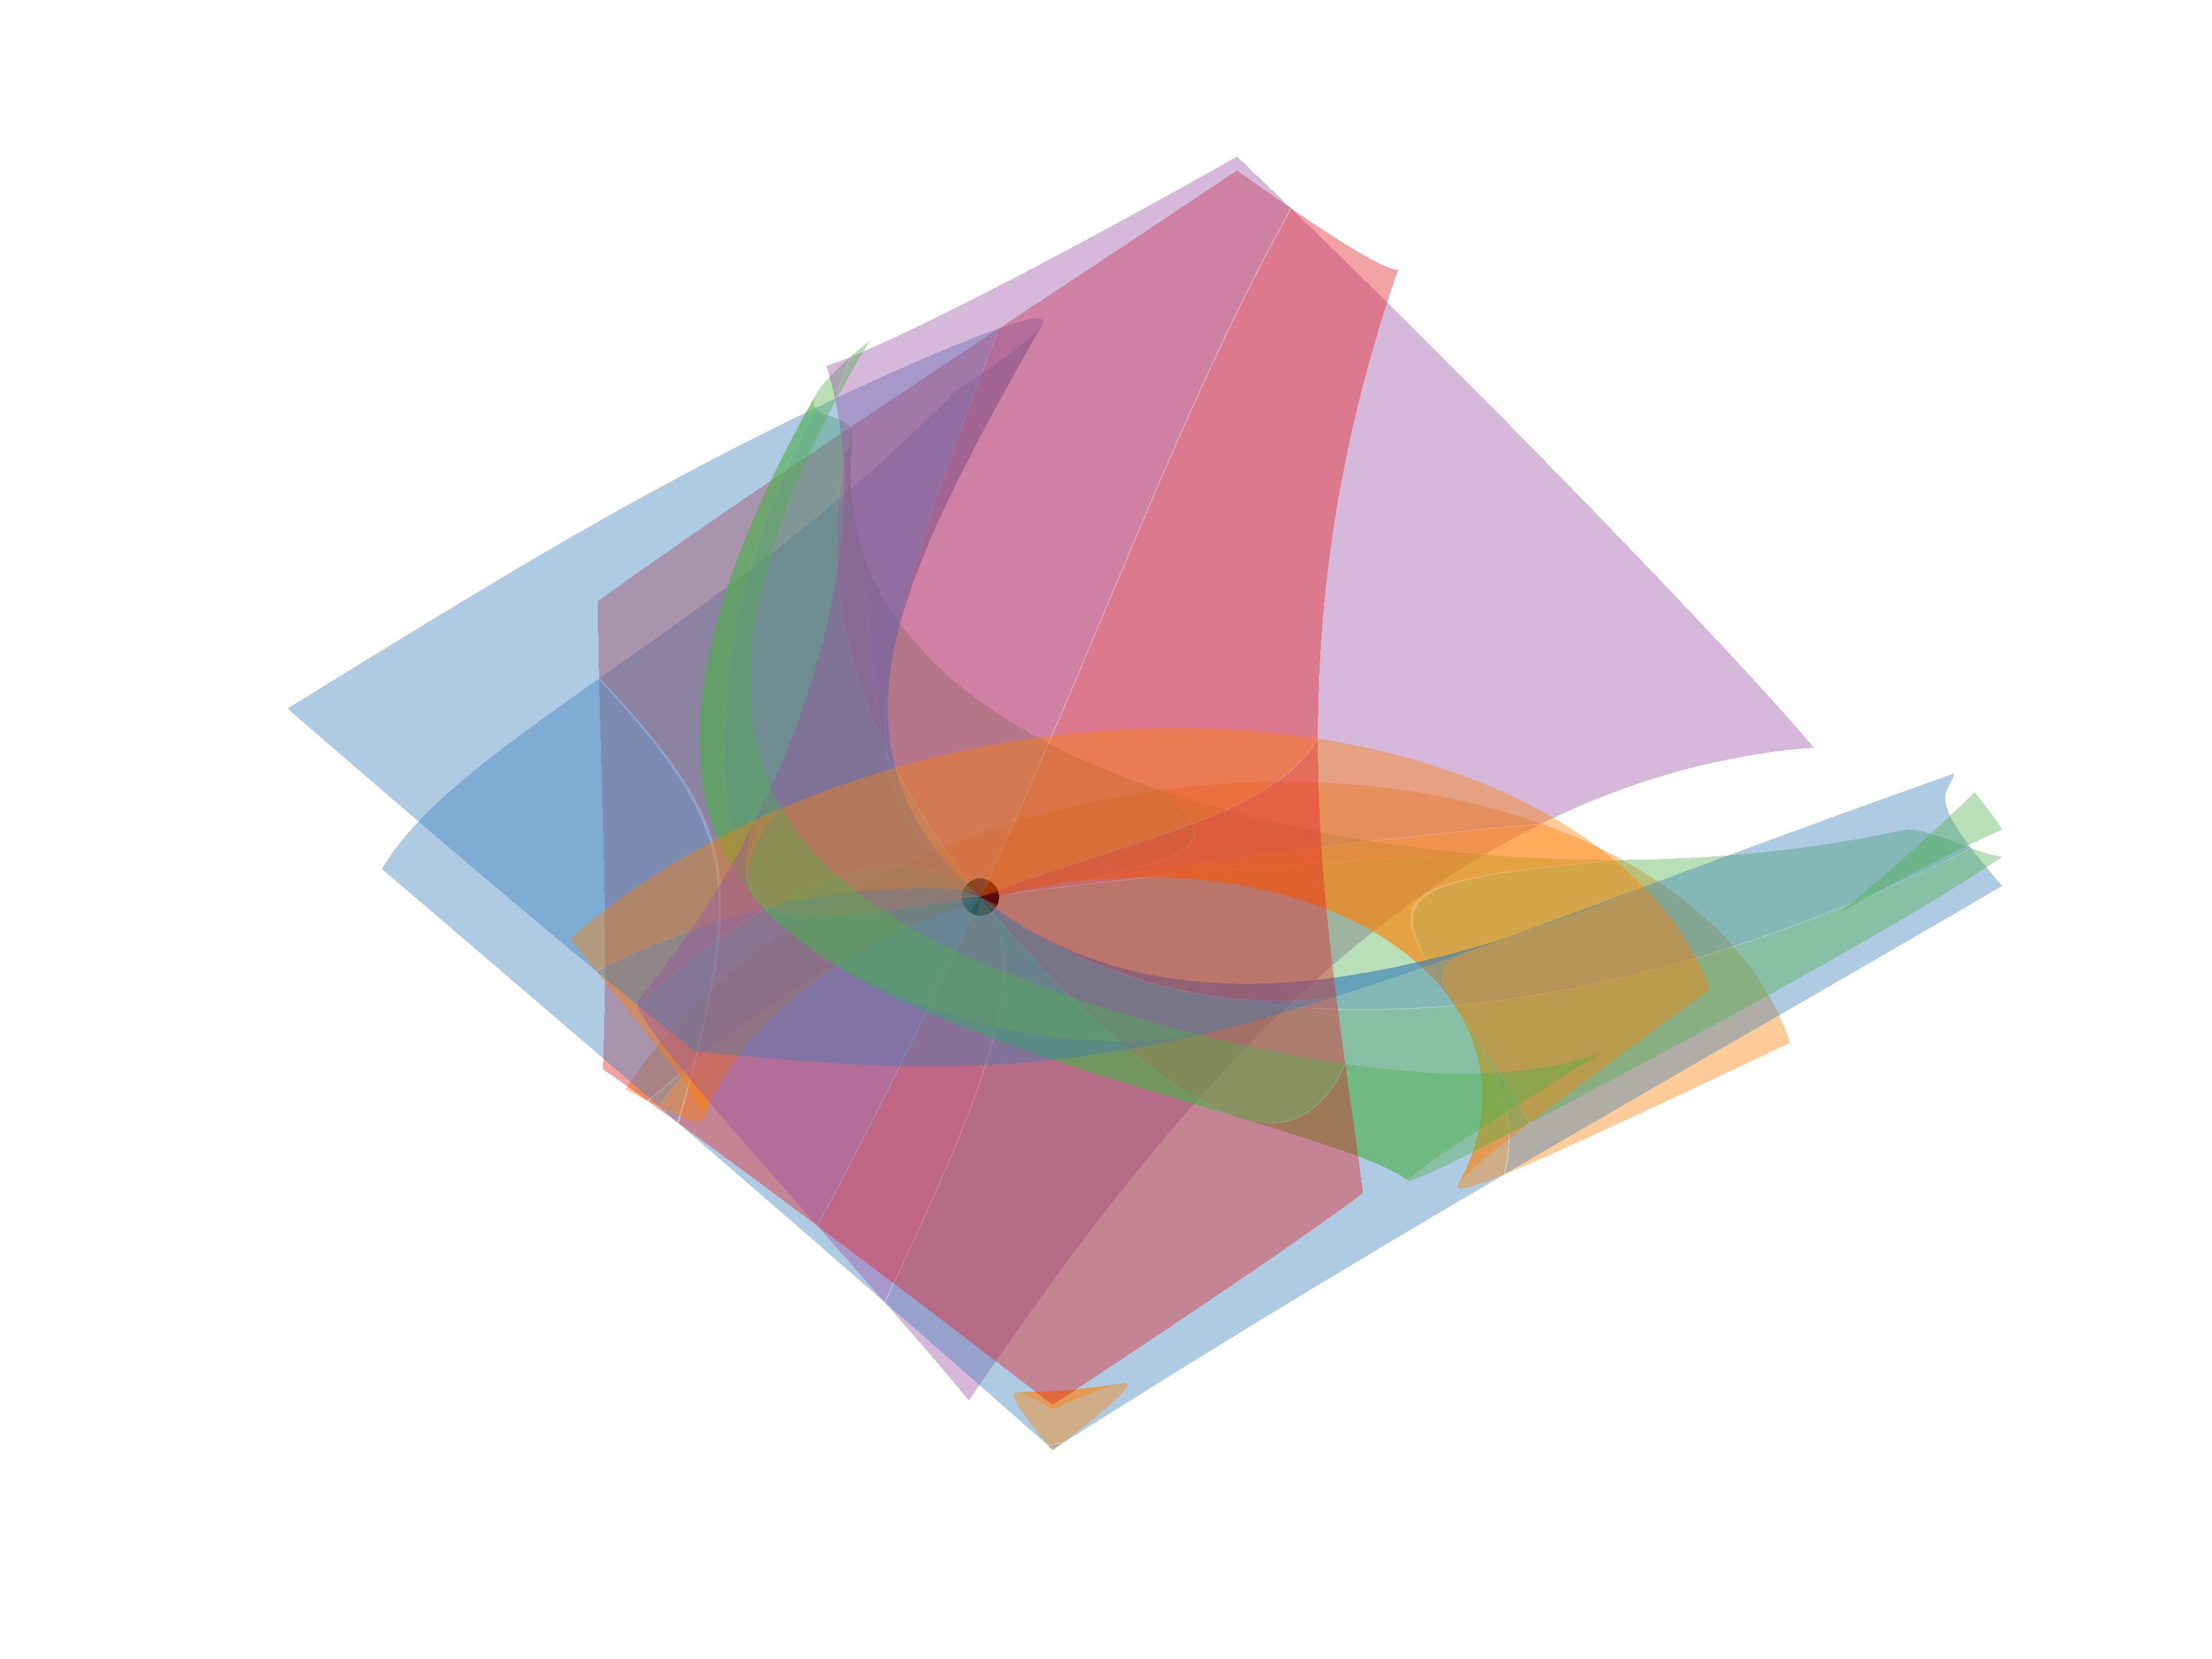
\includegraphics[width=\textwidth]{"images/e5c3_example1_angle.png"}
			\end{subfigure}
			\caption{Die fünf kubischen Hyperflächen aus System \eqref{eqn:example5C3_1}.}
		\end{figure}
	\end{frame}
	\section{Ein 4C3-Algorithmus}
	\begin{frame}
		\frametitle{4C3-Algorithmus}
		\begin{itemize}
			\item Wir wählen die Gruppen $\{X_{2}^3,X_{3}^3,X_{2}^2X_{3},X_{2}X_{3}^2,\}$ und $\{X_{2}^2,X_{2}X_{3},X_{3}^2,X_{2},X_{3},1\}$.\\ \pause
			
			\item Teilen wir jetzt die Koeffizientenmatrix $C$ auf beide Gruppen auf ergibt sich 
			\begin{equation*}
				\small
				-A
				\begin{pmatrix}
					X_{2}^3\\
					X_{2}^2X_{3}\\
					X_{2}X_{3}^2\\
					X_{3}^3
				\end{pmatrix}
				=
				\begin{pmatrix}[1.75]
					\vert & \vert &   & \vert\\
					p_{i,1}(X_{1})&p_{i,2}(X_{1})& \ldots&p_{i,6}(X_{1})\\
					\vert & \vert & & \vert
				\end{pmatrix}
				\begin{pmatrix}
					X_{2}^2\\
					X_{2}X_{3}\\
					X_{3}^2\\
					X_{2}\\
					X_{3}\\
					1
				\end{pmatrix}.
			\end{equation*}
		\end{itemize}
	\end{frame}
	\begin{frame}
		Auflösen nach $G1$ ergibt das System
		\begin{equation*}
			\begin{pmatrix}
				X_{2}^3\\
				X_{2}^2X_{3}\\
				X_{2}X_{3}^2\\
				X_{3}^3
			\end{pmatrix}
			=
			{\Large \text{P`($X_1$)}} \,
			\begin{pmatrix}
				X_{2}^2\\
				X_{2}X_{3}\\
				X_{3}^2\\
				X_{2}\\
				X_{3}\\
				1
			\end{pmatrix}.
		\end{equation*}
	\end{frame}
	\begin{frame}
			Wählen wir die $6$ Identitäten
			\begin{equation*}
				\begin{alignedat}{3}
					X_{3}^3&	\left( X_{2}^3\right)  &=& \left( X_{2}^2X_{3}\right) 	\left( X_{2}X_{3}^2\right), \\
					X_{3}&\left( X_{2}^3\right) &=&\left( X_{2}^2X_{3}\right) X_{2},\\
					X_{3}^2&	\left( X_{2}^3\right)  &=& \left(  X_{2}X_{3}^2\right) 	X_{2}^2,\\
					X_{2}&	\left( X_{3}^3\right)  &=& \left( X_{2}X_{3}^2\right) 	X_{3},\\
					X_{2}^3&	\left( X_{2}X_{3}^2\right)  &=& \left( X_{2}^2X_{3}\right)\left( X_{2}^2X_{3}\right),\\
					X_{3}^3&	\left( X_{2}^2X_{3}\right)  &=& \left( X_{2}X_{3}^2\right)\left( X_{2}X_{3}^2\right),\\
				\end{alignedat}
			\end{equation*}
			\pause
			so erfüllen diese \textbf{\textcolor{red}{nicht}} die Voraussetzungen für eine erfolgreiche Substitution.
	\end{frame}
	\begin{frame}
		\begin{itemize}
			\item Die Polynome
			$p'_{i,j}(X_{1})$ für $i \in \{1,2,3,4\}, \ j \in \{1,2,3\}$ müssen das Nullpolynom sein.
			\pause
			\item Da aber $\det(A) \neq 0$ gilt, müssen schon alle $p_{i,j}(X_{1})$ für $i \in \{1,2,3,4\}, \ j \in \{1,2,3\}$ Nullpolynome sein.
		\end{itemize}
	\end{frame}
	\begin{frame}
				\begin{itemize}
			\item Aus dem resultierenden System
			\begin{equation*}
				M(X_{1})\cdot\begin{pmatrix}[1.3]
					X_{2}^2,
					X_{2}X_{3},
					X_{3}^2,
					X_{2},
					X_{3},
					1
				\end{pmatrix}^\top=0
			\end{equation*}
			erhalten wir über die Determinante von $M(X_{1})$ Lösungskandidaten.
			\item Da dies kein lineares Gleichungssystem ist, lösen wir erst das lineare System
			\begin{equation*}\label{eqn:low_rank_system_ind}
				\tilde{M} \cdot\begin{pmatrix}
					s,
					t,
					u,
					v,
					w,
					1
				\end{pmatrix}^\top
				=0.
			\end{equation*}
			\item Die Lösung dieses Systems ist ein $(5-r)$-dimensionaler affiner Unterraum, der Gestalt ${v_0 + U \subset K^6}$.
			\item Unsere Lösungen sind dann die Elemente des Schnitts \begin{equation*}
				v_0 + U \bigcap \{(v^2,v\cdot w,w^2,v,w,1) : v,w \in K\}
			\end{equation*}
		\end{itemize}
	\end{frame}
	\subsection*{Beispiel}
	\begin{frame}
		\begin{exm}\label{ex:4C3_1}
			Betrachten wir das Gleichungssystem
			\begin{equation*}\label{eqn:example4C3_1}
				\begin{alignedat}{-1}
					2\,x+2\,y+3\,z-x\,y+5\,x\,z-4\,x^2\,z+5\,x^3-y^3-3&=0,\\ x-4\,y-4\,z+4\,x\,y-4\,x\,z+2\,x^2\,y+x^2\,z-y^2\,z-3\,x^3+4&=0,\\ x^2\,y-4\,y-2\,z-2\,x\,y-4\,x\,z-3\,x-4\,x^2\,z-y\,z^2-x^3+2&=0,\\ 3\,x-3\,y-2\,z+x\,y-4\,x\,z+2\,x^2\,y+4\,x^2\,z+4\,x^3-z^3+3&=0
				\end{alignedat}
			\end{equation*}
			über $\R$ so erhalten wir mit dem 4C3-Algorithmus die Lösung
			\begin{equation*}
				\begin{alignedat}{5}
					&\left( x_{1},y_{1},z_{1}\right) &=& \left(0, 0, 1 \right).&&
				\end{alignedat}
			\end{equation*}
		\end{exm}
			\end{frame}
		\begin{frame}
		\begin{figure}[H]
			\begin{subfigure}[b]{0.8\textwidth}
				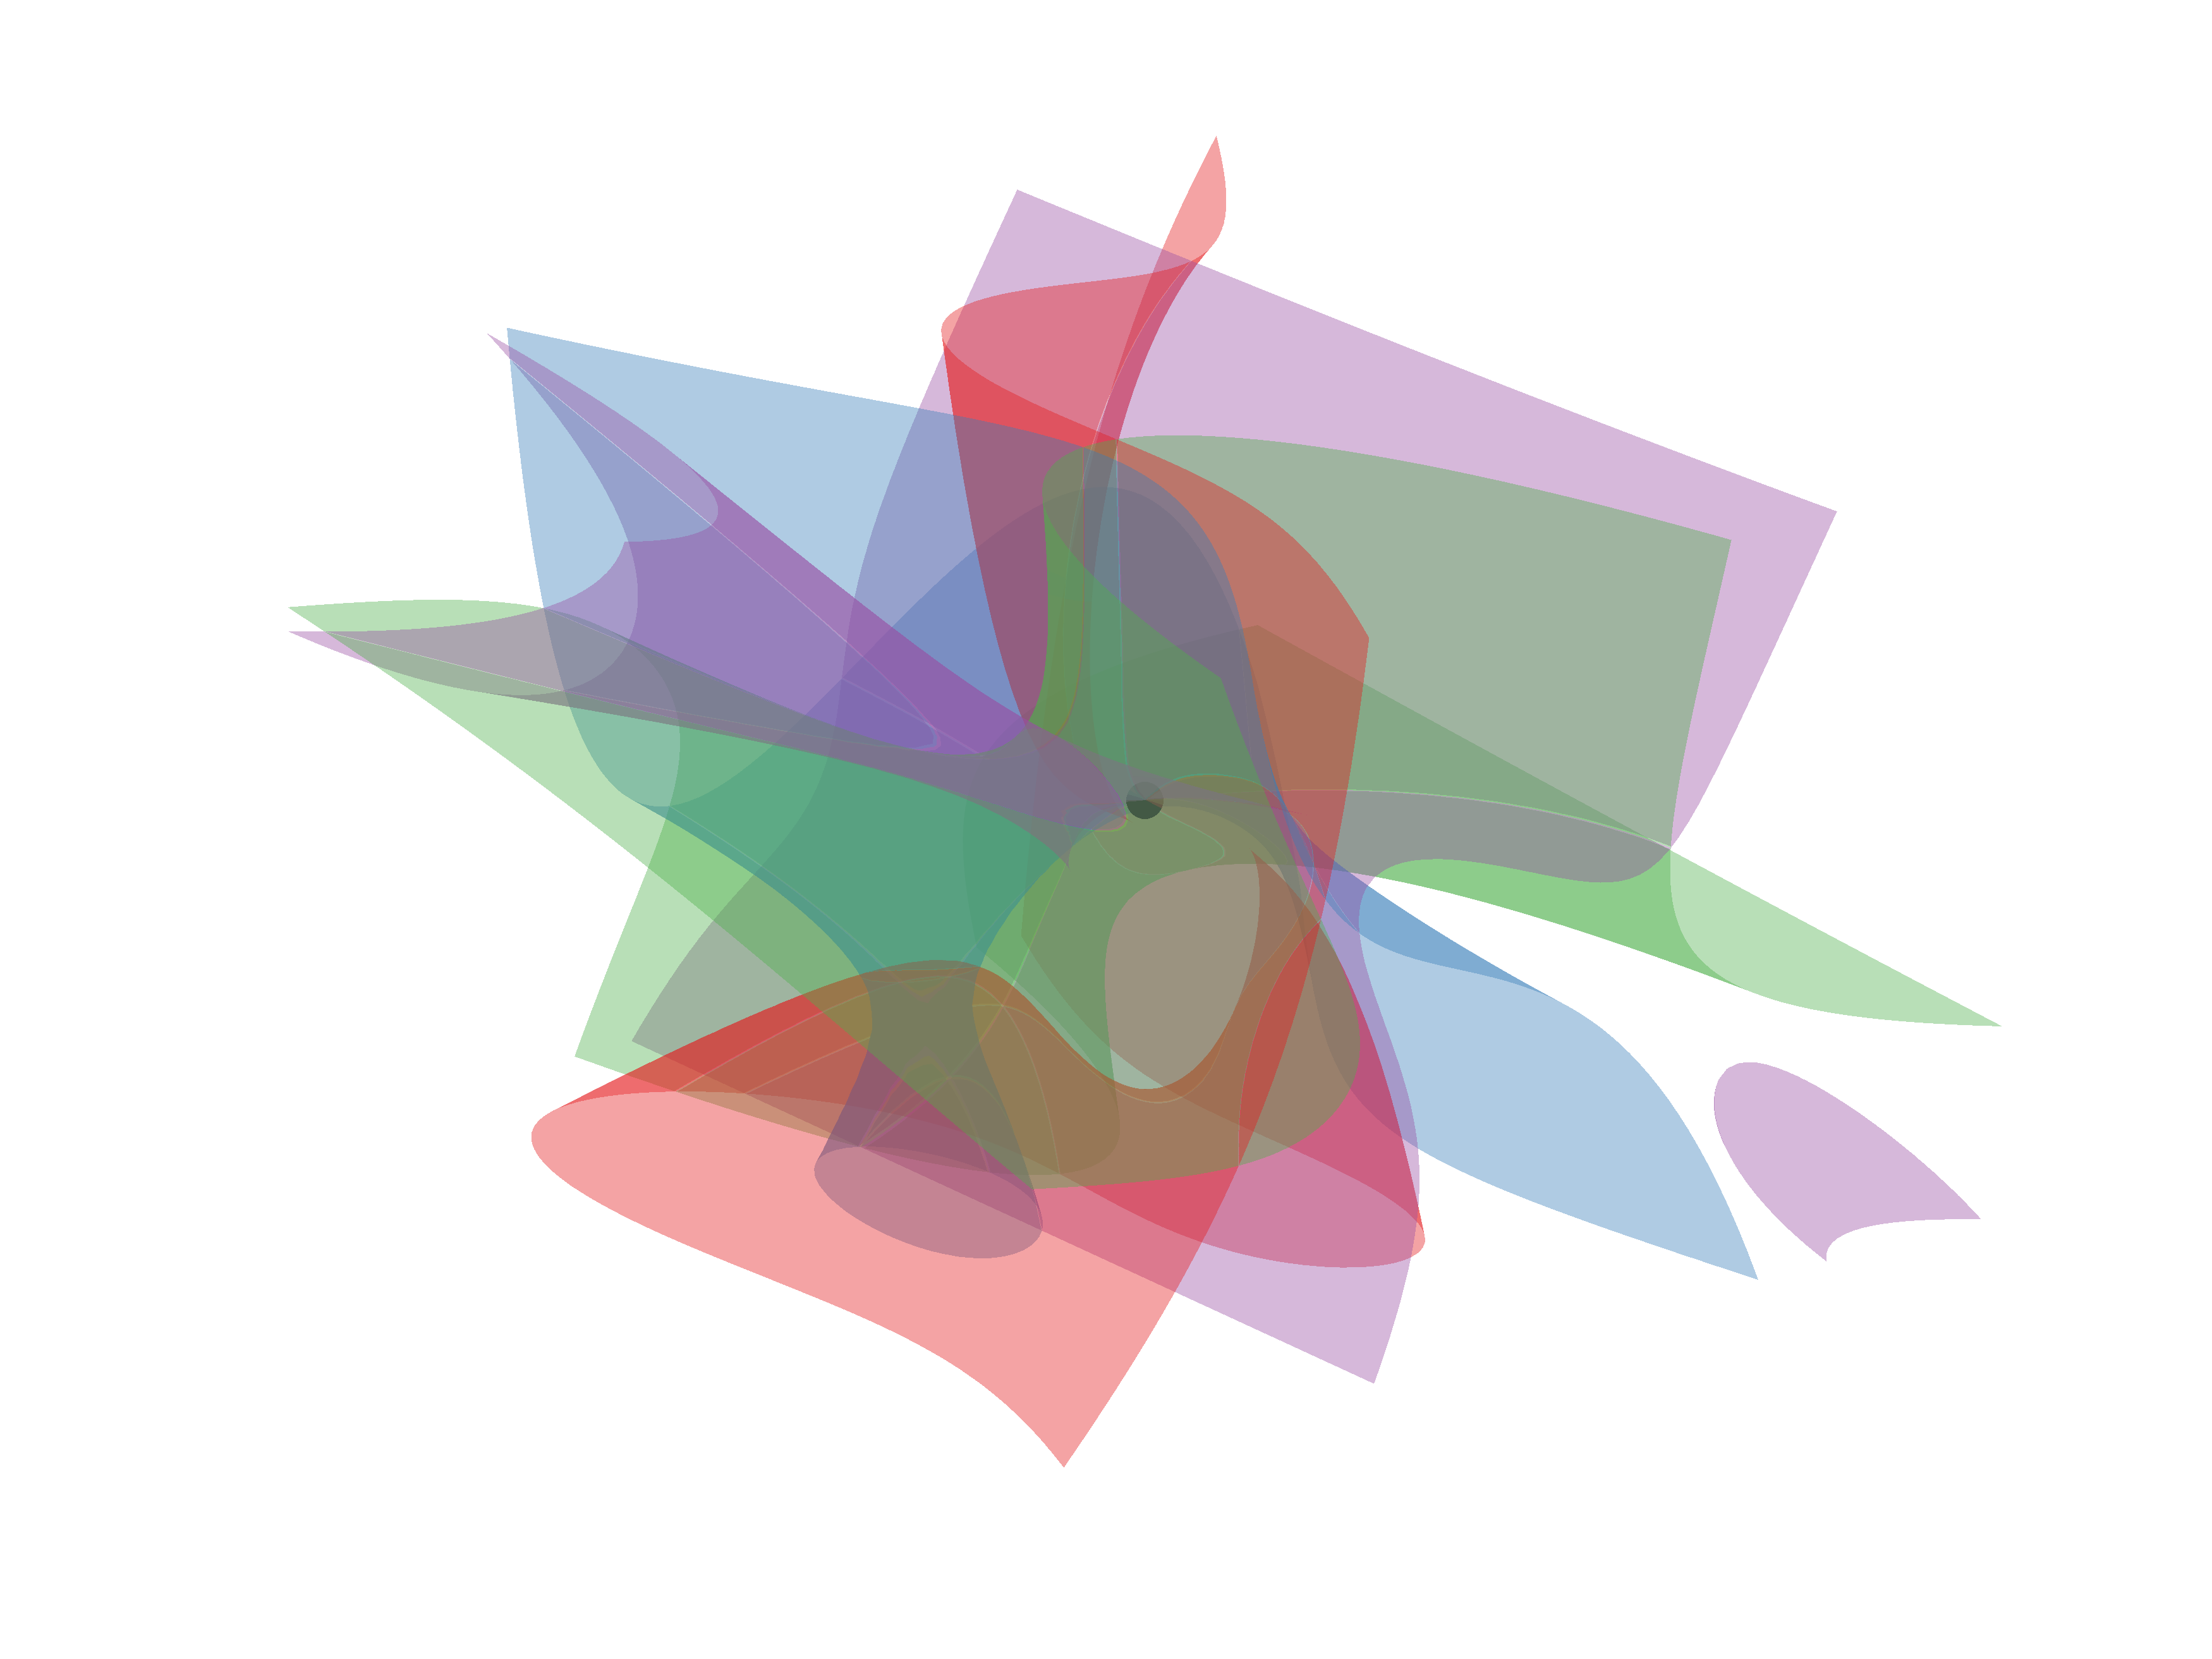
\includegraphics[width=\textwidth]{"images/e4c3_example1.png"}
				\subcaption{Die vier kubischen Flächen (rot,blau,grün und lila) und deren gemeinsamer Schnittpunkt.}
			\end{subfigure}
		\end{figure}
	\end{frame}
	\section{Ein 3C3-Algorithmus}
	\begin{frame}
		\frametitle{3C3-Algorithmus}
		\begin{itemize}
			\item Wir wählen die Gruppen $\{X_{2}^3,X_{2}^2X_{3},X_{2}X_{3}\}$ und $\{X_{2}X_{3}^2,X_{3}^3,X_{2}^2,X_{3}^2,X_{2},X_{3},1\}$.\\ \pause
			
			\item Teilen wir jetzt die Koeffizientenmatrix $C$ auf beide Gruppen auf ergibt sich 
			\begin{equation*}
				-A
				\begin{pmatrix}[2]
			X_{2}^3\\
X_{2}^2X_{3}\\
X_{2}X_{3}
				\end{pmatrix}
				=
				\begin{pmatrix}[1.75]
					\vert & \vert &   & \vert\\
					p_{i,1}(X_{1})&p_{i,2}(X_{1})& \ldots&p_{i,7}(X_{1})\\
					\vert & \vert & & \vert
				\end{pmatrix}
				\begin{pmatrix}
			X_{2}X_{3}^2\\
X_{3}^3\\
X_{2}^2\\
X_{3}^2\\
X_{2}\\
X_{3}\\
1
				\end{pmatrix}.
			\end{equation*}
		\end{itemize}
	\end{frame}
	\begin{frame}
		Auflösen nach $G1$ ergibt das System
		\begin{equation*}
			\begin{pmatrix}[2]
X_{2}^3\\
X_{2}^2X_{3}\\
X_{2}X_{3}
			\end{pmatrix}
			=
			{\Large \text{P`($X_1$)}} \,
			\begin{pmatrix}
			X_{2}X_{3}^2\\
X_{3}^3\\
X_{2}^2\\
X_{3}^2\\
X_{2}\\
X_{3}\\
1
			\end{pmatrix}.
		\end{equation*}
	\end{frame}
	\begin{frame}
		Wählen wir die $7$ Identitäten
		\begin{equation*}
			\small
		\begin{alignedat}{1}
	X_{2}^{3}\cdot X_{3}	&=  X_{2}^{2}X_{3}\cdot X_{2}, \\
	X_{2}^{3}\cdot X_{3} &=  X_{2}X_{3}\cdot X_{2}^2, \\
	X_{2}^{2}X_{3} \cdot X_{3}	&= X_{2}X_{3} \cdot X_{2}X_{3}, \\
	X_{2}^{3}\cdot X_{3}^3 	&=  X_{2}^{2}X_{3}\cdot X_{2}X_{3}^2, \\
	X_{2}^{3}\cdot X_{3}^3	&=  X_{2}X_{3} \cdot X_{2}X_{3} \cdot X_{2}X_{3}, \\
	X_{2}^{3}\cdot X_{3}^2 	&=  X_{2}^{2}X_{3}\cdot X_{2}X_{3},\\
	X_{2}^{2} X_{3} 	&=  X_{2}X_{3}\cdot X_{2}.
\end{alignedat}
		\end{equation*}
		\pause
		so erfüllen diese \textbf{\textcolor{red}{nicht}} die Voraussetzungen für eine erfolgreiche Substitution.\\
		\pause
		Auch das Ausschließen quadratischer Terme analog zum $4C3$-Fall reicht \textbf{\textcolor{red}{nicht}} aus.
	\end{frame}
	\begin{frame}
			\begin{itemize}
				\item Also fordern wir, dass alle Polynome
				$p'_{i,j}(X_{1})$ für $i \in \{1,2,3\}, \ j \in \{1,2,3,4,5,6\}$ das Nullpolynom sind.
				\pause
				\item Analog zum $4C3$-Fall müssen schon alle $p_{i,j}(X_{1})$ für $i \in \{1,2,3\}, \ j \in \{1,2,3,4,5,6\}$ Nullpolynome sein.
				\pause
				\item Weiter gilt
				\begin{equation*}
					X_{2}X_{3}^2 = X_{2}X_{3} \cdot X_{3}
				\end{equation*}
				gilt und weil wir $X_{2}X_{3}$ substituieren kommt das Monom nach Substitution nicht vor.\\
				Wir können also eine Identität weglassen.
			\end{itemize}
	\end{frame}
	\begin{frame}
		\begin{itemize}
			\item Wir erhalten also das System
			\begin{equation*}
			\tilde{M}\begin{pmatrix}[1.3]
				X_{2}^2,
				X_{2}X_{3},
				X_{3}^2,
				X_{2},
				X_{3},
				1
			\end{pmatrix}^{\top} =0
			\end{equation*}
			erhalten wir über die Determinante von $M(X_{1})$ Lösungskandidaten.
			\item Da dies kein lineares Gleichungssystem ist, lösen wir analog erst das lineare System
			\begin{equation*}\label{eqn:low_rank_system_ind}
				\tilde{M} \cdot\begin{pmatrix}
					s,
					t,
					u,
					v,
					w,
					1
				\end{pmatrix}^\top
				=0.
			\end{equation*}
			\item Die Lösung dieses Systems ist ein $(5-r)$-dimensionaler affiner Unterraum, der Gestalt ${v_0 + U \subset K^6}$.
			\item Unsere Lösungen sind dann die Elemente des Schnitts \begin{equation*}
				v_0 + U \bigcap \{(w^3,v^2,w^2,v,w,1) : v,w \in K\}
			\end{equation*}
		\end{itemize}
	\end{frame}
	\subsection*{Beispiele}
	\begin{frame}
		\begin{exm}
			\begin{equation*}\label{eqn:example3C3_1}
				\small
				\begin{alignedat}{-1}
    x^3+4.5430\,x^2+7.5462\,x+5\,y^3-4\,z\,y^2-13.1784\,z\,y+51.6952&=0\\ 4\,x^3+15.1718\,x^2+20.0987\,x+4\,y^3+z\,y^2+4.5446\,z\,y+22.4914&=0\\ 2\,x^3+8.0859\,x^2+11.7303\,x-2\,y^3+5\,z\,y^2+18.7231\,z\,y-37.0671&=0
				\end{alignedat}
			\end{equation*}
		\end{exm}
	\end{frame}
		\begin{frame}
		\begin{exm}
			\begin{equation*}\label{eqn:example3C3_1}
				\small
				\begin{alignedat}{-1}
					x^3+4.5430\,x^2+7.5462\,x+5\,y^3-4\,z\,y^2-13.1784\,z\,y+51.6952&=0\\ 4\,x^3+15.1718\,x^2+20.0987\,x+4\,y^3+z\,y^2+4.5446\,z\,y+22.4914&=0\\ 2\,x^3+8.0859\,x^2+11.7303\,x-2\,y^3+5\,z\,y^2+18.7231\,z\,y-37.0671&=0
				\end{alignedat}
			\end{equation*}
		\end{exm}
	\end{frame}
		\begin{frame}
		\begin{exm}
			\begin{equation*}\label{eqn:example3C3_1}
				\small
				\begin{alignedat}{-1}
 x^3+55588\,x^2+77685\,x+5\,y^3+99992\,z\,y^2+92749\,z\,y+90961&=0\\
  7\,x^3+89101\,x^2+21432\,x+y^3+z\,y^2+18839\,z\,y+51045&=0\\
   2\,x^3+11172\,x^2+18308\,x+100001\,y^3+5\,z\,y^2+94208\,z\,y+73380&=0
				\end{alignedat}
			\end{equation*}
			über $\F{100003}$.
		\end{exm}
	\end{frame}
	\section{Programme}
	\begin{frame}
		\frametitle{Programmlaufzeit}
		Im Falle endlicher Körper $\F{p}$ stellen sich für den $E3Q3$ und $3C3$-Algorithmus zwei Fragen:\pause
		\begin{enumerate}
			\item[1.] Wie verhält sich die Laufzeit bei steigender Ordnung $p$?\pause
			\item[2.] Ist der Algorithmus besser als jede Möglichkeit auszuprobieren?
		\end{enumerate}
	\end{frame}
	\begin{frame}
		\frametitle{Ist der Algorithmus besser als jede Möglichkeit auszuprobieren?}
		\begin{figure}[H]
			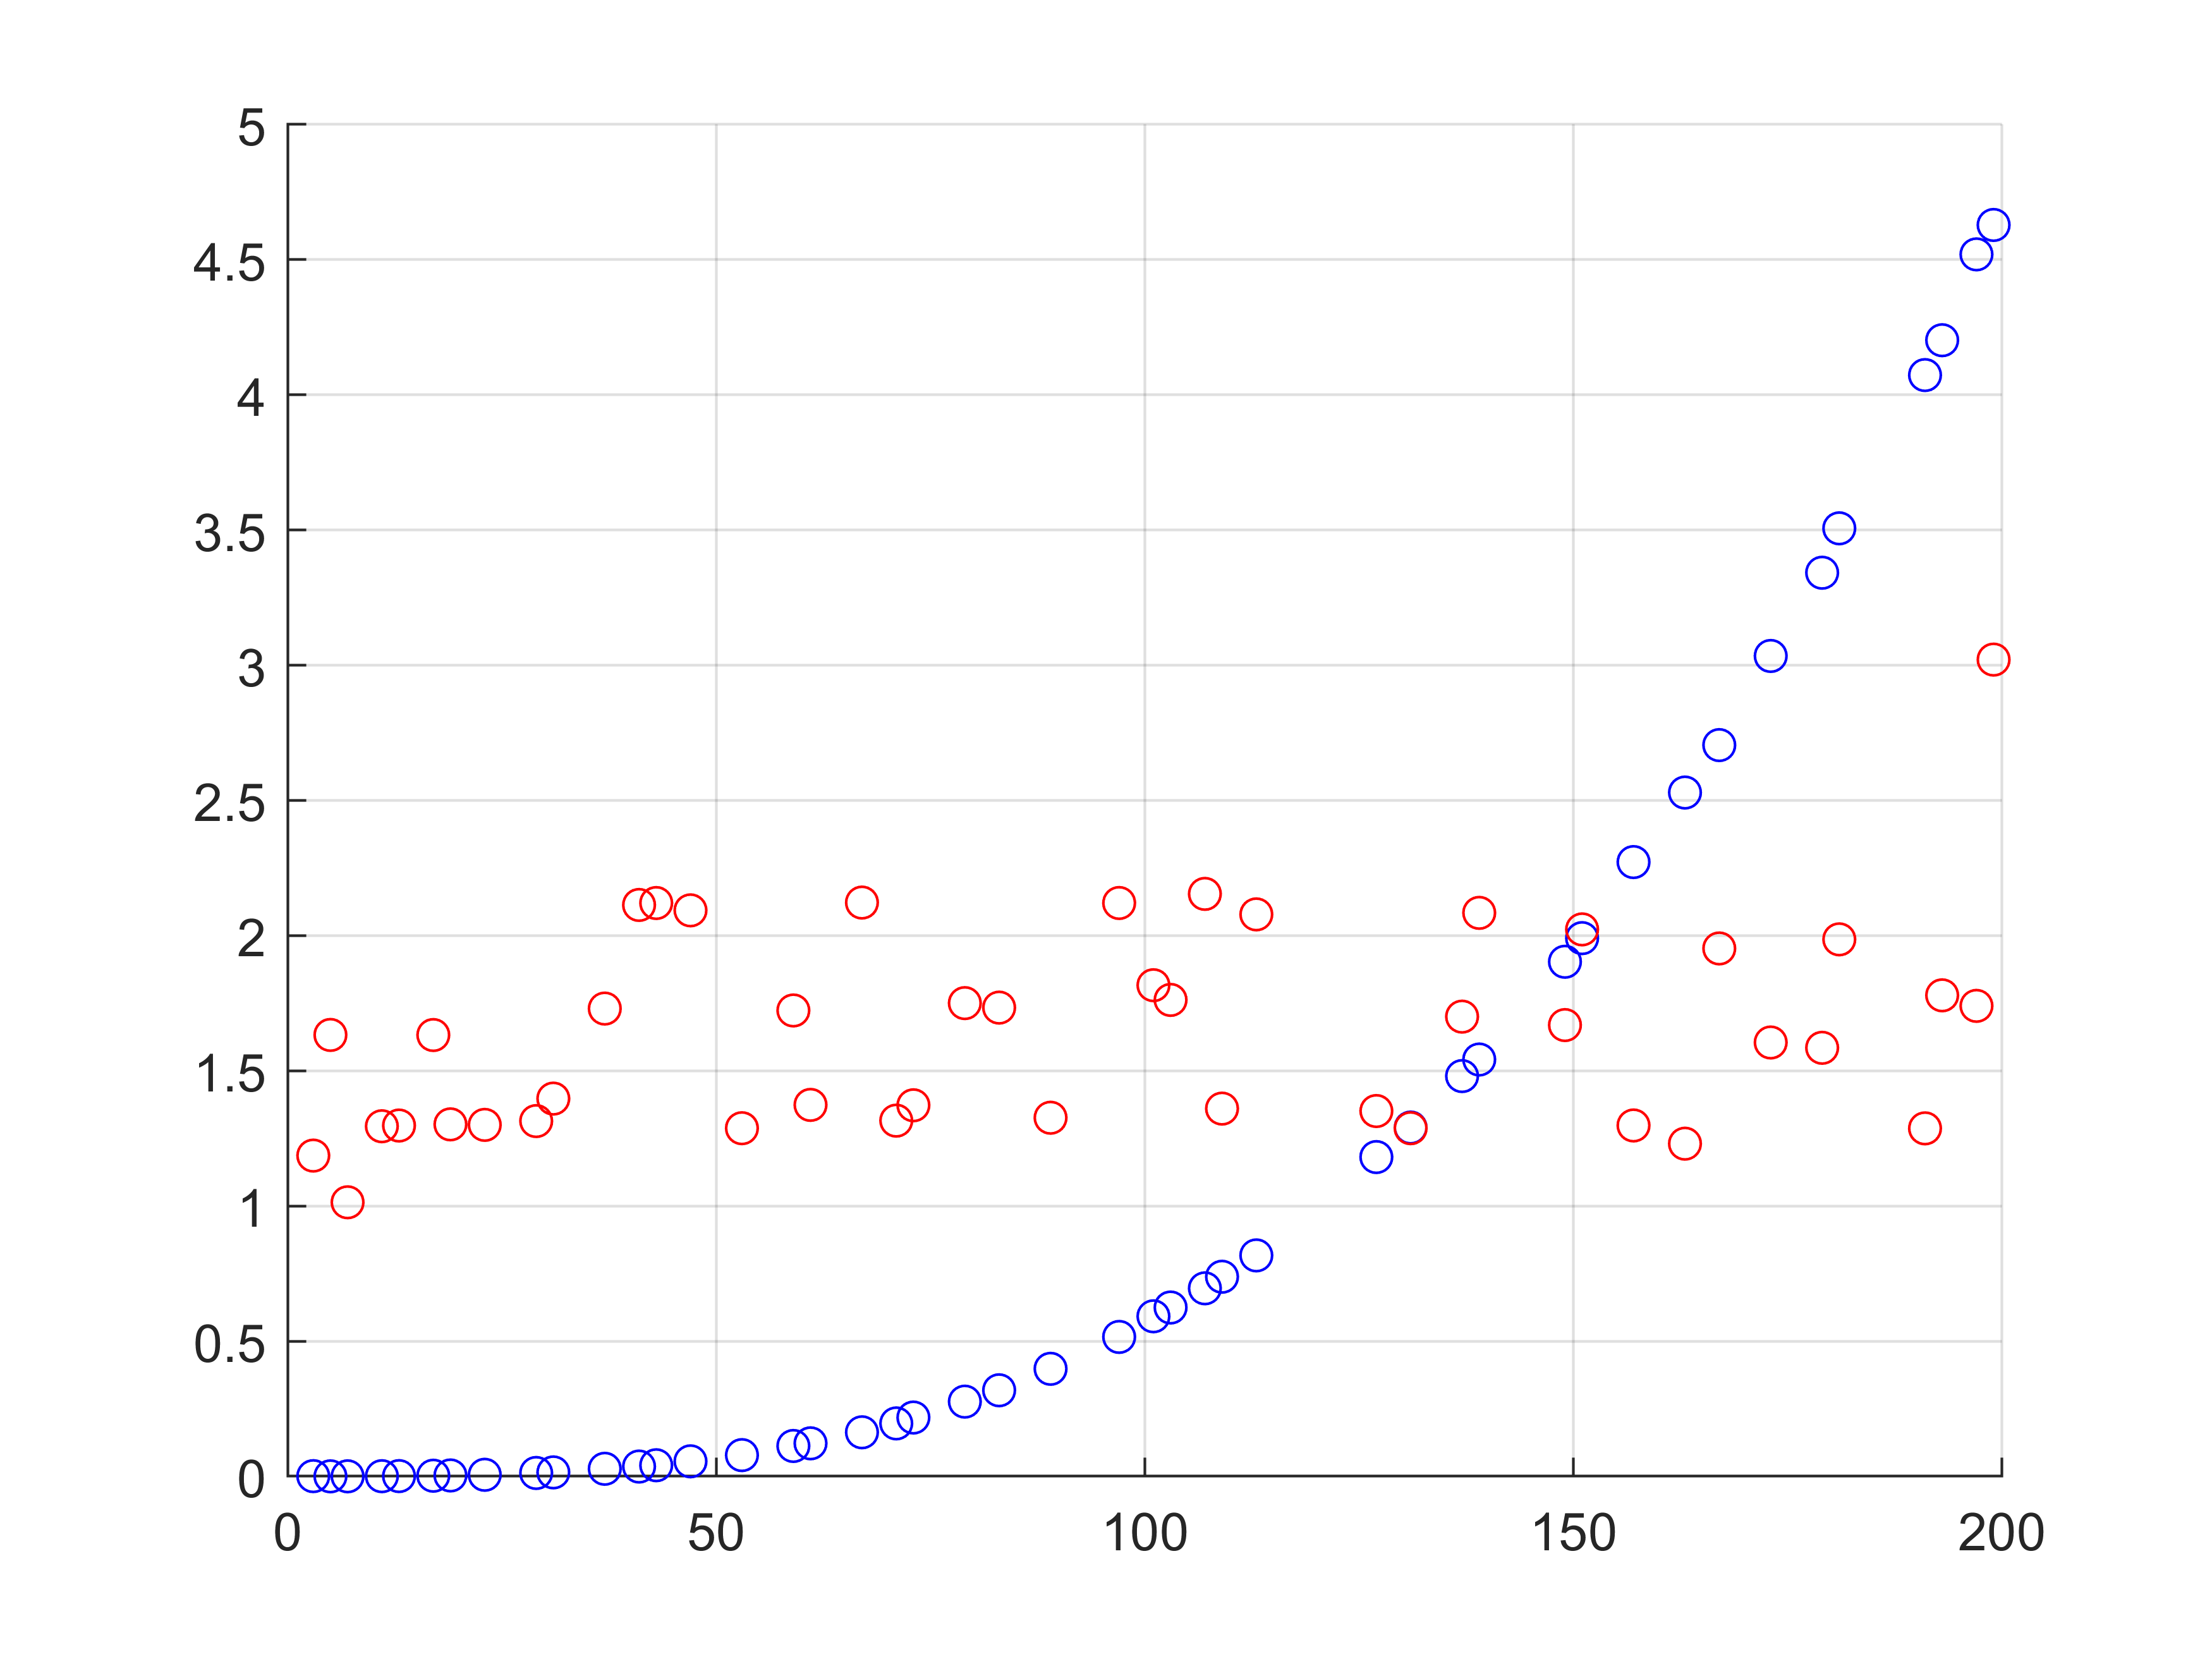
\includegraphics[width=0.65\textwidth]{"images/runtime_e3q3_for_loop.png"}
			\caption*{Durchschnittliche Laufzeit des E3Q3-Algorithmus (rot) und For-Loop (blau)}
		\end{figure}
	\end{frame}
	\begin{frame}
		\frametitle{Ist der Algorithmus besser als jede Möglichkeit auszuprobieren?}
		\begin{figure}[H]
			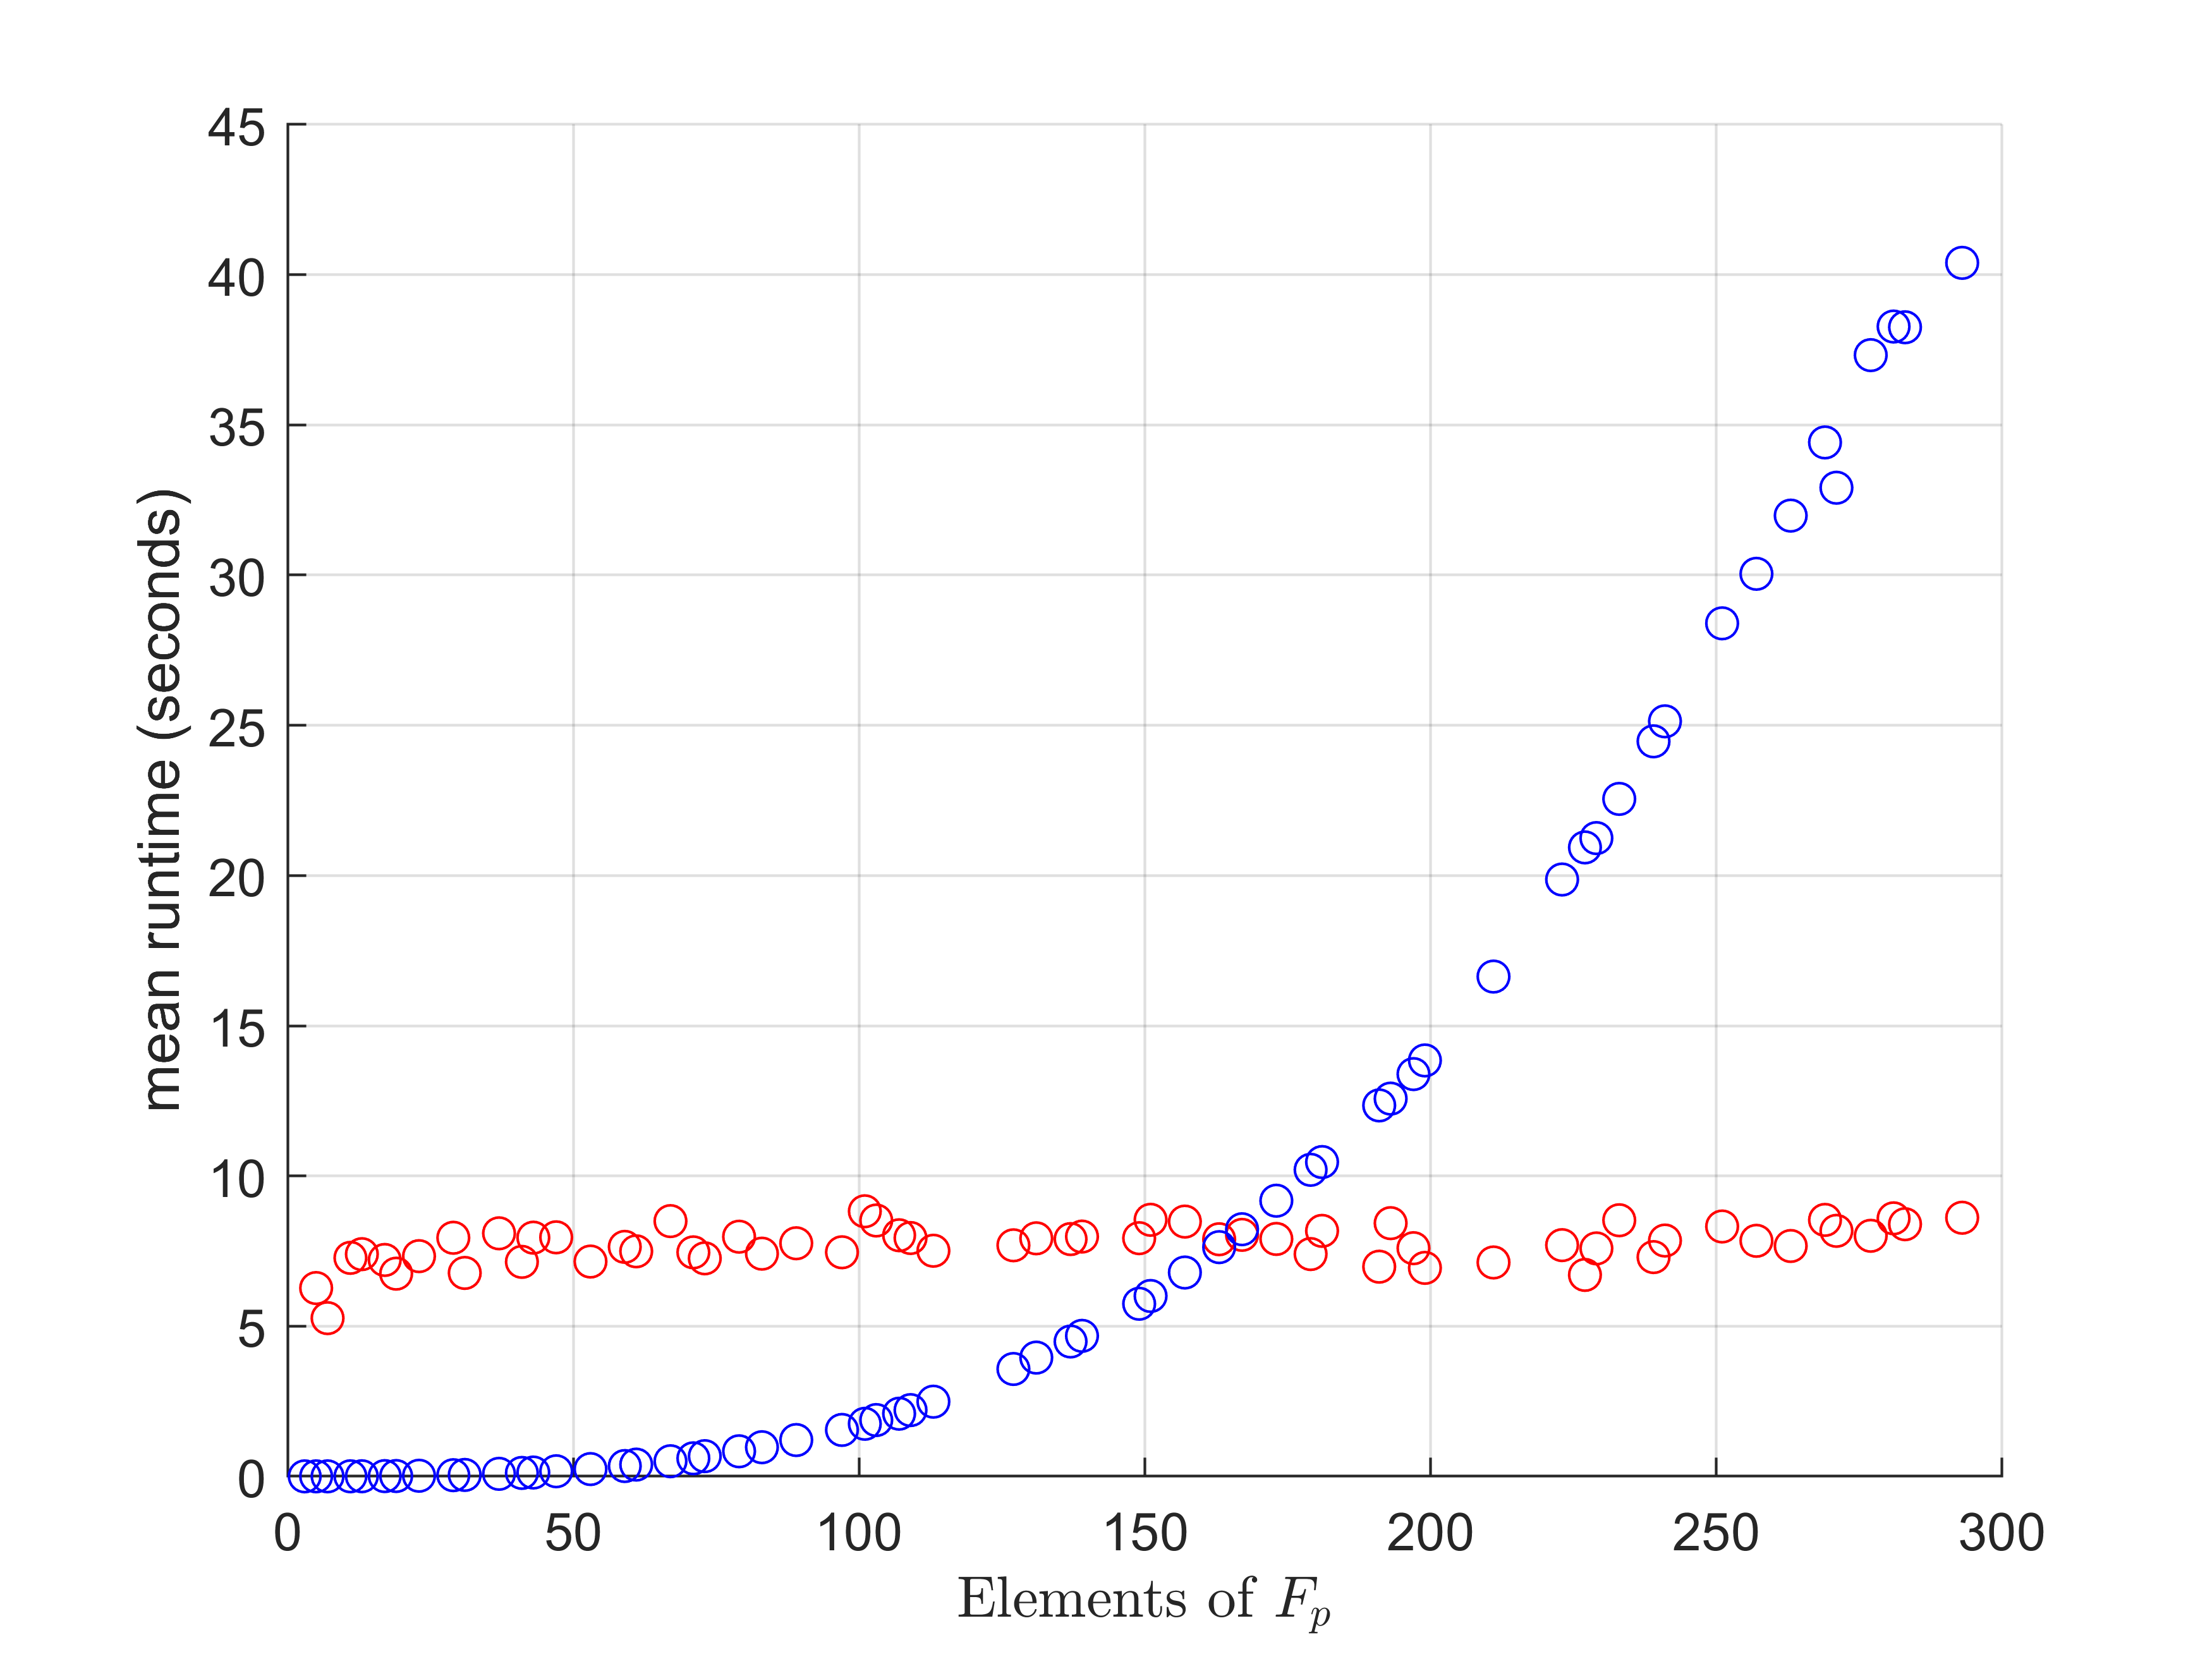
\includegraphics[width=0.65\textwidth]{"images/runtime_e3c3_for_loop_2.png"}
			\caption*{Durchschnittliche Laufzeit des E3C3-Algorithmus (rot) und For-Loop (blau)}
		\end{figure}
	\end{frame}
	\begin{frame}
		\frametitle{Wie verhält sich die Laufzeit bei steigender Ordnung $p$?}
		\begin{figure}[H]
			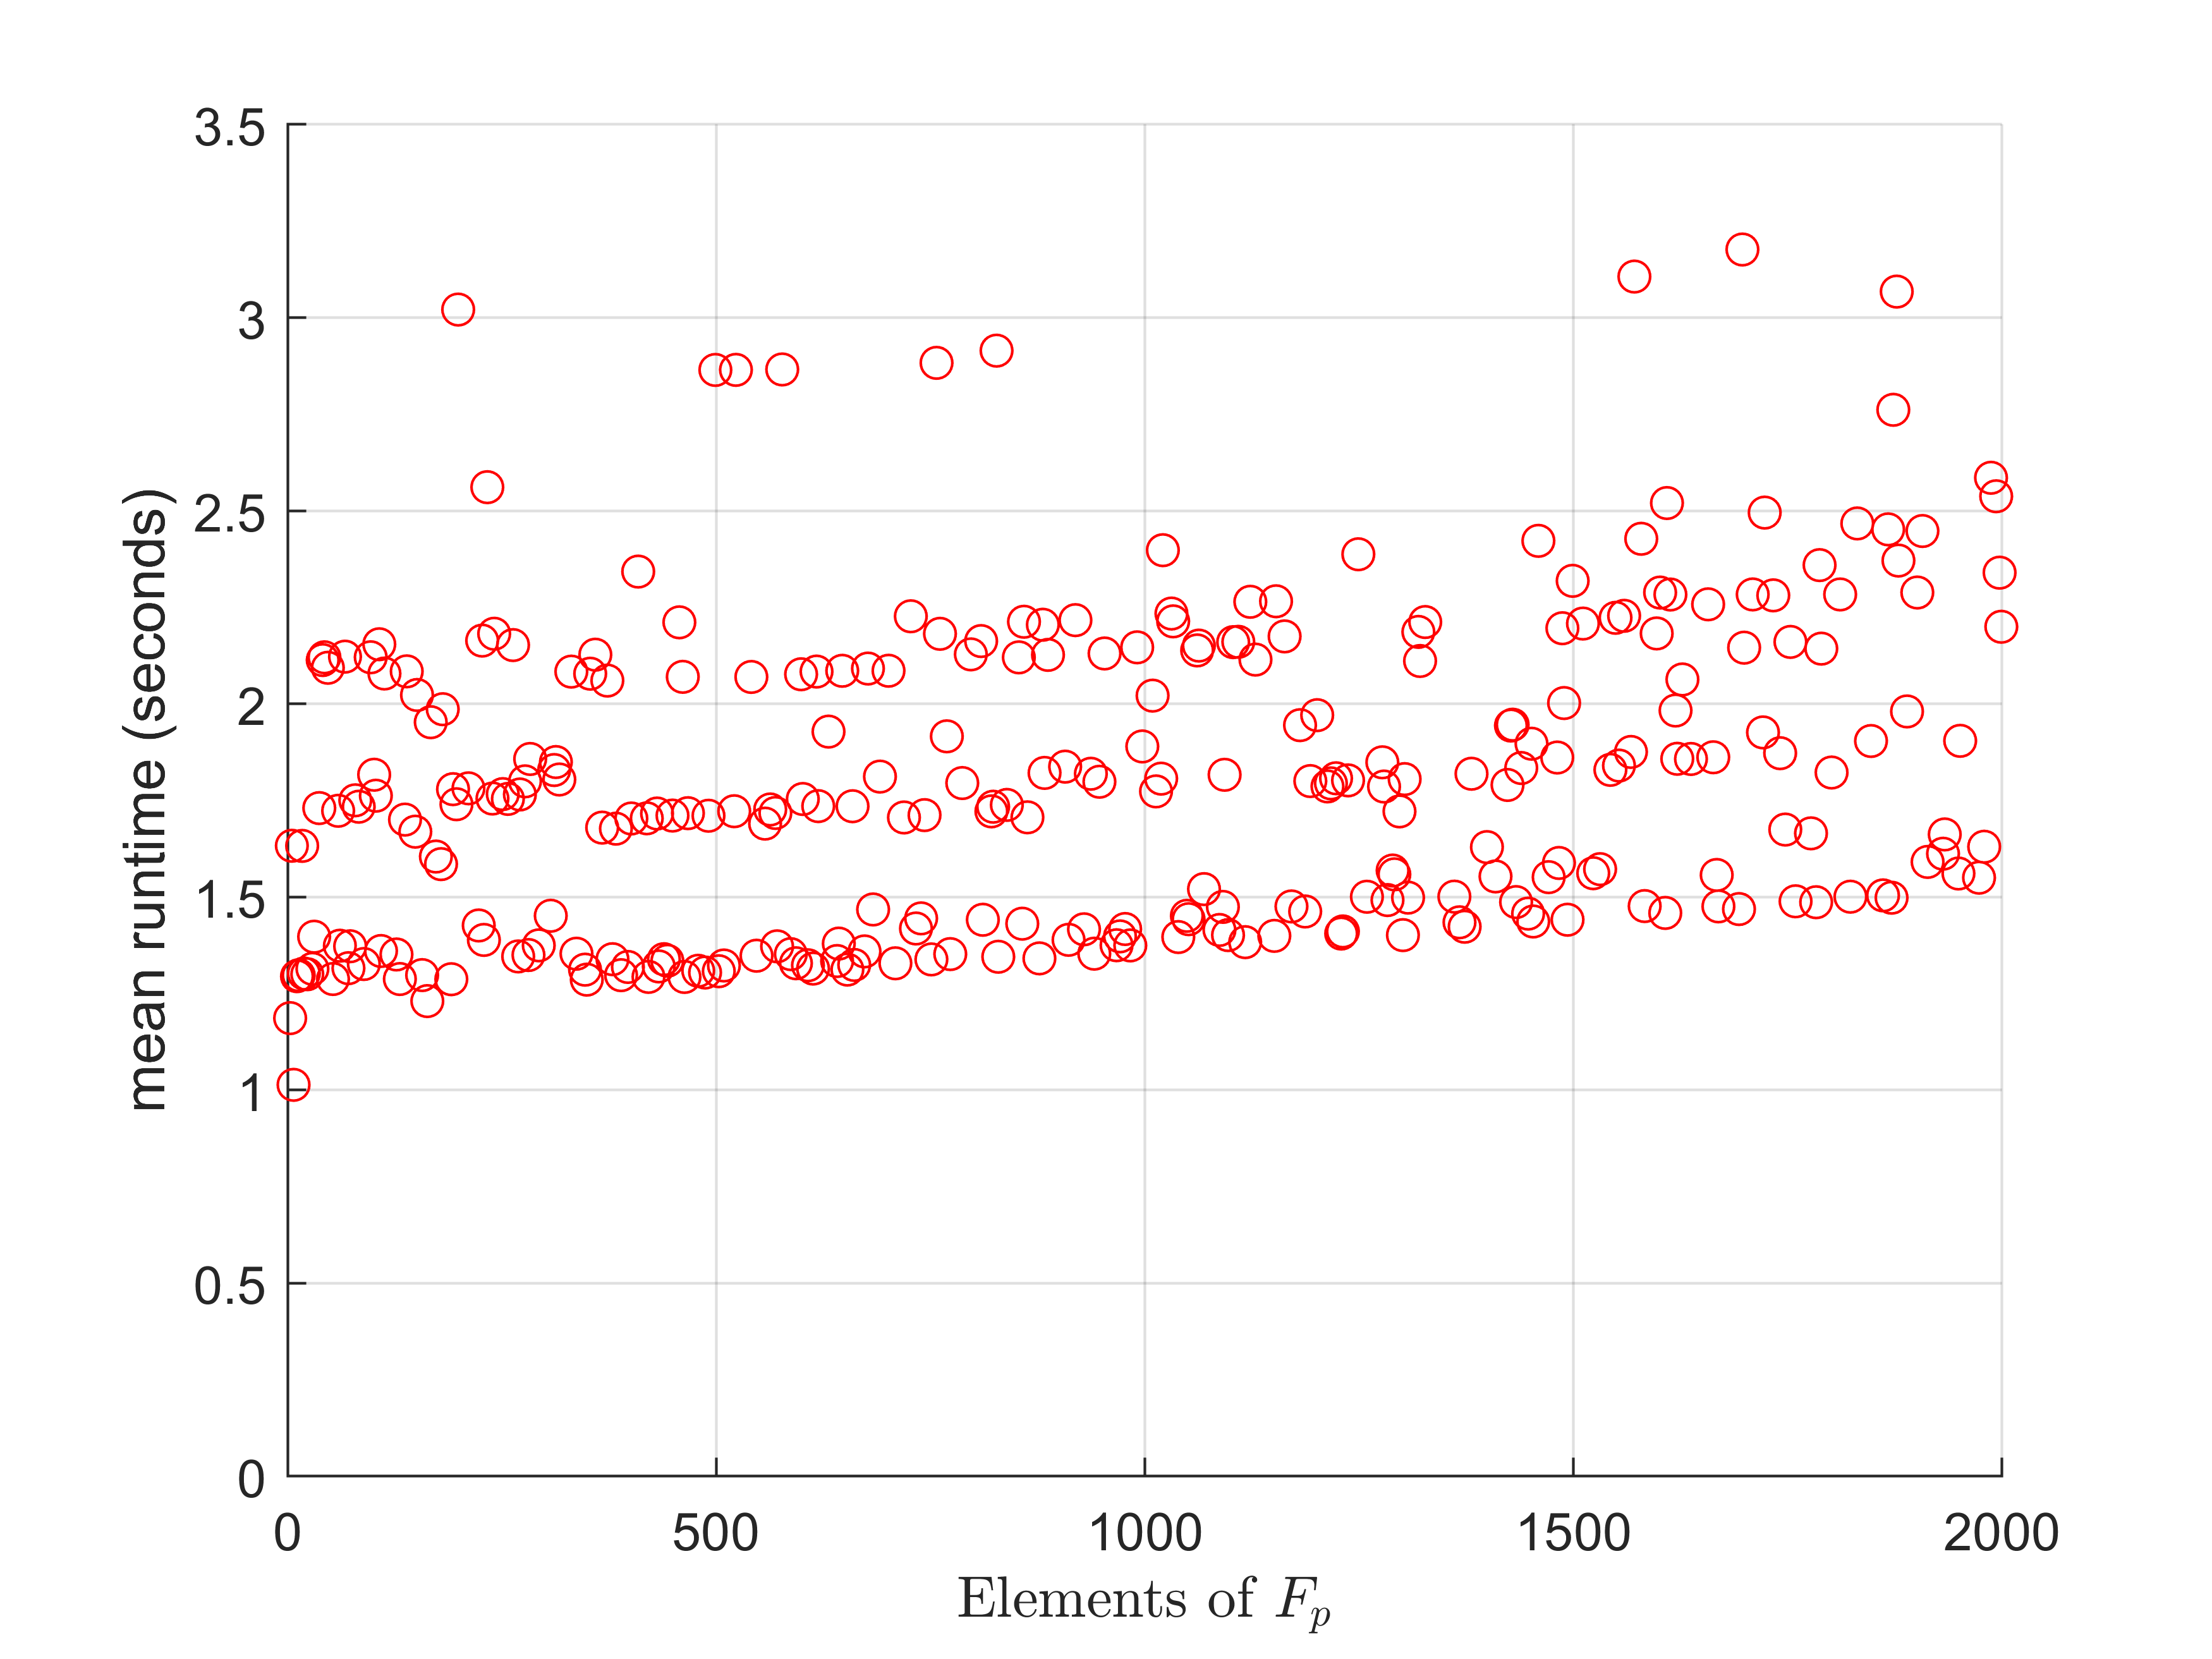
\includegraphics[width=0.7\textwidth]{"images/runtime_e3q3.png"}
			\caption{Durchschnittliche Laufzeit des E3Q3-Algorithmus}
		\end{figure}
	\end{frame}
	\begin{frame}
		\frametitle{Wie verhält sich die Laufzeit bei steigender Ordnung $p$?}
		\begin{figure}[H]
			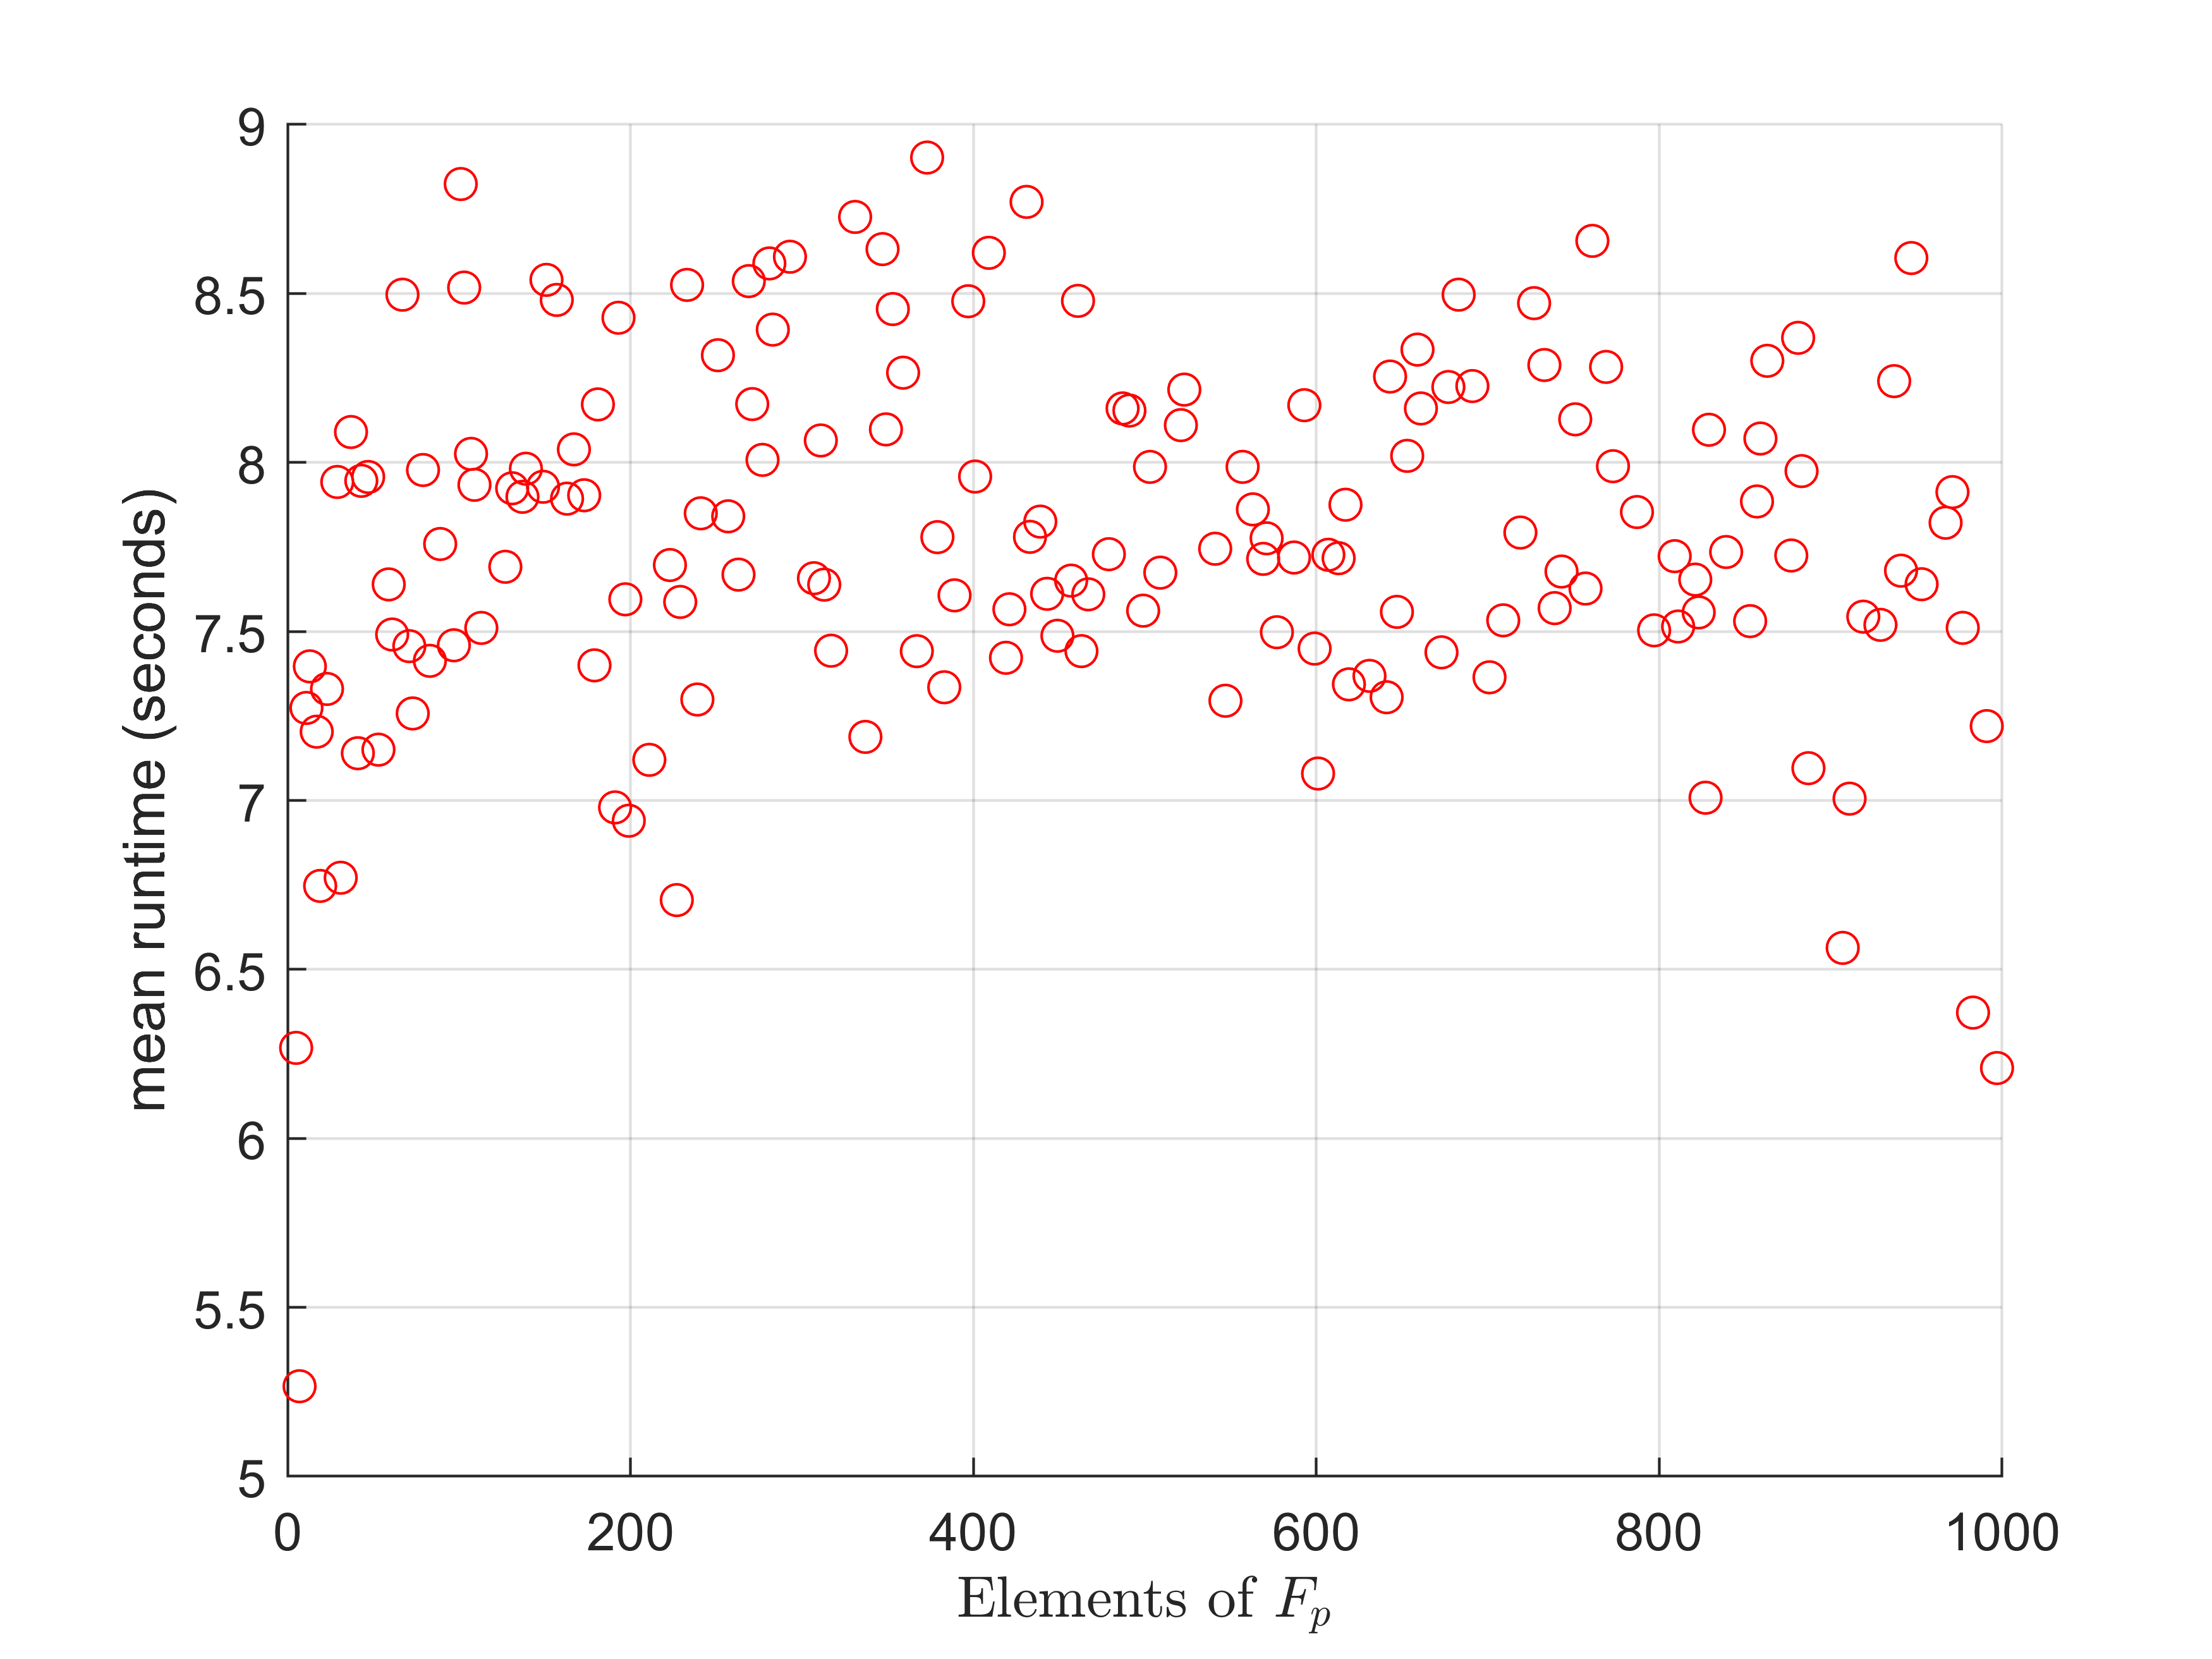
\includegraphics[width=0.7\textwidth]{"images/runtime_e3c3_2.png"}
			\caption{Durchschnittliche Laufzeit des E3C3-Algorithmus}
		\end{figure}
	\end{frame}
	\section{Fazit}
	\begin{frame}
		\begin{itemize}
			\frametitle{Fazit}
			\pause
			\item Wir haben erfolgreich den E3Q3-Algorithmus über den reellen Zahlen und endlichen Körpern mit Primordnung implementiert.
			\pause
			\item Außerdem konnten wir den Algorithmus auch auf den Fall dreier kubischer Flächen formulieren, wobei wir die Koeffizienten der Flächen einschränken mussten.
		\end{itemize}
	\end{frame}
	\section{Ausblick}
	\begin{frame}
		\begin{itemize}
			\frametitle{Ausblick}
			\pause
			\item Im 3C3-Algorithmus kann die Nullmatrix auftaucht. In den anderen Algorithmen korrespondierte dies damit, dass der Lösungskandidat $\tilde{x}_1$ keine Lösung war. Im 3C3-Algorithmus führt dies aber zu dass jedes Element der Menge \begin{equation*}
				\{(\tilde{x}_i,0,z) \ \forall z \in K\}
			\end{equation*}
			eine Lösung ist. Hier ist nicht klar, ob aus dem Auftreten der Nullmatrix immer diese Lösungsmenge folgt.
			\pause
			\item \textbf{TODO} Auch könnte es neben $G_1=\{X_2^3,X_2^2X_3,X_2X_3\}$ und $G_1=\{X_2^3,X_2^2X_3,X_2X_3^2\}$ noch weitere Aufteilungen der Monome geben, für welche sich passende Identitäten für einen weiteren 3C3-Algorithmus formulieren lassen.
		\end{itemize}
	\end{frame}
	\section*{}
	\begin{frame}
		\begin{center}
			\huge \textcolor{blue}{Danke für eure Aufmerksamkeit!}
		\end{center}
	\end{frame}
		\begin{frame}
		\begin{center}
			\huge \textcolor{blue}{Fragen und/oder Gleichungssysteme?}
		\end{center}
	\end{frame}
		\begin{frame}
				\bibliographystyle{ieeetr}
			\nocite{*}
			\bibliography{bibliography.bib}
	\end{frame}
\end{document}